\documentclass[10pt,aspectratio=169]{beamer}

\usetheme{metropolis}
\metroset{block=fill,numbering=fraction,progressbar=frametitle}

\usepackage[T1]{fontenc}
\usepackage[utf8]{inputenc}
\IfFileExists{lmodern.sty}{\usepackage{lmodern}}{}
\usepackage{amsmath,amssymb,amsfonts}
\usepackage{mathtools}
\usepackage{booktabs}
\usepackage{tikz}
\usetikzlibrary{arrows.meta,positioning,calc,shapes.geometric,fit,backgrounds}
\usepackage{listings}
\usepackage{xcolor}
\usepackage{graphicx}
\usepackage{animate}

\definecolor{codekw}{RGB}{0,102,153}
\definecolor{codestr}{RGB}{153,51,0}
\definecolor{codecom}{RGB}{110,110,110}
\lstset{language=Python,basicstyle=\ttfamily\scriptsize,
    keywordstyle=\color{codekw}\bfseries,stringstyle=\color{codestr},
    commentstyle=\color{codecom}\itshape,showstringspaces=false,
    columns=fullflexible,breaklines=true,frame=none,aboveskip=2pt,belowskip=2pt}

\newcommand{\R}{\mathbb{R}}
\newcommand{\bF}{\mathbb{F}}
\newcommand{\VR}{\mathrm{VR}}
\newcommand{\Cechsym}{\check{\mathrm{C}}}
\newcommand{\Dgm}{\mathrm{Dgm}}
\newcommand{\dB}{d_{\mathrm{B}}}
\newcommand{\dH}{d_{\mathrm{H}}}
\newcommand{\Tau}{\mathcal{T}}  %
\newcommand{\im}{\operatorname{im}}
\newcommand{\rank}{\operatorname{rank}}
\newcommand{\nullity}{\operatorname{nullity}}
\newcommand{\diam}{\operatorname{diam}}
\newcommand{\HL}[1]{\textcolor{blue!70!black}{#1}}

\graphicspath{{output/}}

\newif\ifcomputedslides
\computedslidestrue

\newcommand{\figmissing}[1]{%
    \fbox{\parbox[c][0.4\textheight][c]{0.8\linewidth}{\centering\scriptsize
    \texttt{\detokenize{output/#1.png}} has not been generated yet.
    \par\vspace{0.6em}
    Run \texttt{python run\_examples.py -{}-talk} from the project root.}}}

\newcommand{\figcredit}[1]{%
        {\scriptsize\textcolor{gray}{computed by \texttt{examples/#1}}}}

\newcommand{\computedfig}[4][0.60]{%
    \begin{center}
    \IfFileExists{output/#2.png}
    {\includegraphics[width=\textwidth,height=#1\textheight,keepaspectratio]{#2}}
    {\figmissing{#2}}
    \end{center}
    \vspace{-0.1em}
    {\footnotesize #3\par}
    \vspace{0.2em}
    \figcredit{#4}%
}

\newcommand{\computedfigside}[4][0.62]{%
    \begin{columns}[c,onlytextwidth]
    \begin{column}{#1\textwidth}
    \centering
    \IfFileExists{output/#2.png}
    {\includegraphics[width=\linewidth,height=0.80\textheight,keepaspectratio]{#2}}
    {\figmissing{#2}}
    \end{column}
    \begin{column}{\dimexpr0.95\textwidth-#1\textwidth\relax}
    \scriptsize #3
    \vspace{0.8em}
    \par\figcredit{#4}
    \end{column}
    \end{columns}%
}

\newcommand{\hexpoints}{%
    \foreach \i/\a in {1/0,2/60,3/120,4/180,5/240,6/300}{\coordinate (P\i) at (\a:1.5);}}
\newcommand{\hexdots}{\foreach \i in {1,...,6}{\fill[black] (P\i) circle (2pt);}}

\newcommand{\spinetriangle}[1]{%
    \begin{tikzpicture}[scale=1.15]
    \coordinate (a) at (0,0); \coordinate (b) at (1.5,0); \coordinate (c) at (0.75,1.25);
    #1
    \draw[very thick,-{Stealth[length=2mm]}] (a)--($(a)!0.55!(b)$);
    \draw[very thick] (a)--(b);
    \draw[very thick,-{Stealth[length=2mm]}] (b)--($(b)!0.55!(c)$);
    \draw[very thick] (b)--(c);
    \draw[very thick,-{Stealth[length=2mm]}] (a)--($(a)!0.55!(c)$);
    \draw[very thick] (a)--(c);
    \foreach \p in {a,b,c}{\fill (\p) circle (2.2pt);}
    \node[below left] at (a) {$a$}; \node[below right] at (b) {$b$}; \node[above] at (c) {$c$};
    \node[below,font=\scriptsize] at (0.75,-0.35) {$e_1=ab$, $e_2=bc$, $e_3=ac$};
    \end{tikzpicture}}

\title{Introduction to Topological Data Analysis}
\subtitle{Homology, Laplacian, Betti numbers}
\author{Arystan Shokan}
\institute{Boston University}
\date{\today}

\begin{document}

    \maketitle

    \begin{frame}{Plan}
        \begin{columns}[T,onlytextwidth]
            \begin{column}{0.55\textwidth}
                \footnotesize
                \begin{enumerate}
                    \item \textbf{Motivation}
                    \item \textbf{From points to complexes}
                    \item \textbf{Homology as linear algebra}
                    \item \textbf{Persistence}
                    \item \textbf{Demo: TDA in an AI pipeline}
                    \item \textbf{The Hodge Laplacian}
                    \item \textbf{Wrap-up \& exercise}
                \end{enumerate}
                \vspace{0.2em}
            \end{column}
            \begin{column}{0.42\textwidth}
                \begin{block}{What you need}
                    \scriptsize
                    Kernel, image, rank, and rank--nullity. If you have ever used spectral clustering or
                    a graph convolutional network, you already have more than enough.
                \end{block}

            \end{column}
        \end{columns}
    \end{frame}

    \section{Motivation}

    \begin{frame}{Three data sets your tools cannot tell apart}
        \begin{center}
            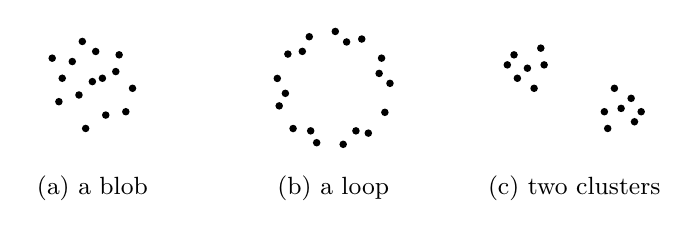
\begin{tikzpicture}[scale=0.85]
\begin{scope}[shift={(0,0)}]
    \foreach \x/\y in {0/0.1,0.4/0.5,-0.3/0.4,0.2/-0.4,-0.5/-0.2,0.6/0.0,-0.1/-0.6,
    0.35/0.25,-0.45/0.15,0.05/0.55,-0.2/-0.1,0.5/-0.35,-0.6/0.45,0.15/0.15,-0.15/0.7}
    \fill[black] (\x,\y) circle (1.6pt);
    \node at (0,-1.5) {\small (a) a blob};
\end{scope}
\begin{scope}[shift={(3.6,0)}]
    \foreach \a in {5,32,60,88,115,143,170,198,225,253,280,308,335} \fill[black] (\a:0.85) circle (1.6pt);
    \foreach \a in {18,74,130,186,242,298} \fill[black] (\a:0.72) circle (1.6pt);
    \node at (0,-1.5) {\small (b) a loop};
\end{scope}
\begin{scope}[shift={(7.2,0)}]
    \foreach \x/\y in {-0.7/0.3,-0.5/0.6,-0.9/0.5,-0.6/0.0,-0.85/0.15,-0.45/0.35,-1.0/0.35}
    \fill[black] (\x,\y) circle (1.6pt);
    \foreach \x/\y in {0.7/-0.3,0.5/-0.6,0.9/-0.5,0.6/0.0,0.85/-0.15,0.45/-0.35,1.0/-0.35}
    \fill[black] (\x,\y) circle (1.6pt);
    \node at (0,-1.5) {\small (c) two clusters};
\end{scope}
            \end{tikzpicture}
        \end{center}
        \vspace{0.2em}
        \small
        Relabel the axes as two coordinates of an embedding, and this is a t-SNE or UMAP plot you have looked at yourself.
        Same mean, near-identical covariance.
        \alert{PCA cannot distinguish (a) from (b).} Let $k$-means pick $k$ by silhouette
        and it answers $k=3$ for all three --- cutting the loop, one connected piece,
        into three arcs.

        \vspace{0.3em}
        \begin{center}
            \alert{Nothing in the standard toolbox has a slot for ``there is a hole in the middle''.}
        \end{center}
    \end{frame}

    \begin{frame}[shrink=8]{Where loops and holes already show up in your work}
        \small
        \begin{itemize}
            \item \textbf{The manifold hypothesis.} Embeddings sit near a low-dimensional manifold in high-dimensional space.
            TDA is the tool that checks this assumption instead of asserting it, and reports \emph{what shape} that manifold has.
            \item \textbf{Generative models.} Mode collapse in a GAN is a connected-components problem: the generator's support has fewer components than the data does.
            Diffusion and VAE latent trajectories that should be periodic trace closed loops --- or fail to.
            \item \textbf{Reinforcement learning.} A policy with cyclic behaviour (a patrol route, a recurring strategy) traces a loop in state or embedding space.
            \item \textbf{Robustness and OOD detection.} Adversarial examples are often pushed
            \emph{off} the data manifold. ``How far is this point from the learned topology of in-distribution data'' is a persistence question.
            \item \textbf{Beyond pairwise graphs.} A GNN message-passing step only sees edges.
            Many relations are genuinely higher-order (a co-authorship triple, a
            three-way interaction) --- exactly what simplicial complexes encode, and the
            reason \emph{topological deep learning} is now an active subfield.
        \end{itemize}

        \vspace{0.2em}
        \begin{center}
            None of this is a linear subspace and none of it is a set of separated clusters.
        \end{center}
    \end{frame}

    \begin{frame}{Betti numbers: counting holes, one dimension at a time}
        \begin{columns}[T,onlytextwidth]
            \begin{column}{0.48\textwidth}
                \footnotesize
                For each $k=0,1,2,\dots$ the \HL{Betti number} $\beta_k$ counts the
                independent $k$-dimensional holes of a shape:
                \begin{itemize}
                    \item $\beta_0$ --- connected pieces;
                    \item $\beta_1$ --- loops: closed curves you cannot shrink to a
                    point, a hole you could thread a string through;
                    \item $\beta_2$ --- enclosed voids: the air inside a ball.
                \end{itemize}

                The data sets from before, as the eye reads them:
                \begin{center}
                    \begin{tabular}{lcc}
                        \toprule
                        & $\beta_0$   & $\beta_1$   \\
                        \midrule
                        (a) a blob       & $1$         & $0$ \\
                        (b) a loop       & $1$         & \alert{$1$} \\
                        (c) two clusters & \alert{$2$} & $0$         \\
                        \bottomrule
                    \end{tabular}
                \end{center}
            \end{column}
            \begin{column}{0.48\textwidth}
                \centering
                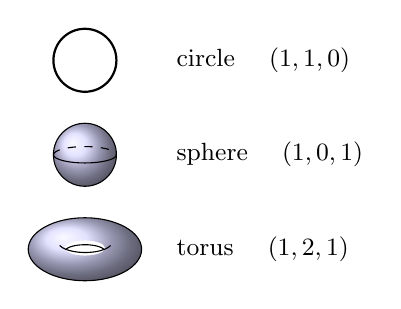
\begin{tikzpicture}[baseline,scale=0.8]
                    \draw[thick] (0,0) circle (0.5);
                    \node[right] at (1.3,0) {\small circle \quad $(1,1,0)$};
                    \begin{scope}[shift={(0,-1.5)}]
                        \shade[ball color=blue!15] (0,0) circle (0.5);
                        \draw (0,0) circle (0.5);
                        \draw (-0.5,0) arc (180:360:0.5 and 0.13);
                        \draw[dashed] (-0.5,0) arc (180:0:0.5 and 0.13);
                        \node[right] at (1.3,0) {\small sphere \quad $(1,0,1)$};
                    \end{scope}
                    \begin{scope}[shift={(0,-3.0)}]
                        \shade[ball color=blue!15, even odd rule]
                        (0,0) ellipse (0.9 and 0.5) (0,0.02) ellipse (0.32 and 0.12);
                        \draw (0,0) ellipse (0.9 and 0.5);
                        \draw (-0.4,0.06) arc (200:340:0.43 and 0.17);
                        \draw (-0.3,0.0) arc (160:20:0.32 and 0.11);
                        \node[right] at (1.3,0) {\small torus \quad $(1,2,1)$};
                    \end{scope}
                \end{tikzpicture}

                \vspace{0.3em}
                {\scriptsize $(\beta_0,\beta_1,\beta_2)$ for each surface. The torus has
                two independent loops: around the tube, and through the hole.\par}
            \end{column}
        \end{columns}

        \vspace{0.3em}
        \centering\small PCA and clustering miss \alert{$\beta_1$} entirely. Part 3 computes these
        numbers as ranks of matrices; Part 4 makes them survive noise.
    \end{frame}

    \begin{frame}[shrink=15]{What we are going to build, and what we are skipping}
        \begin{block}{The goal}
            An invariant $\beta_k$ that counts $k$-dimensional holes, is computed by
            \alert{Gaussian elimination}, and does not change when you deform the data.
        \end{block}

        \vspace{0.4em}
        \begin{columns}[T,onlytextwidth]
            \begin{column}{0.47\textwidth}
                \begin{block}{We will do}
                    \scriptsize
                    \begin{itemize}
                        \item complexes from point clouds / embeddings
                        \item boundary matrices, $\ker$ and $\im$
                        \item Betti numbers by rank--nullity
                        \item persistence and stability
                        \item the Hodge Laplacian: the graph
                        Laplacian you already know, one level up
                    \end{itemize}
                \end{block}
            \end{column}
            \begin{column}{0.47\textwidth}
                \begin{block}{We will skip, on purpose}
                    \scriptsize
                    \begin{itemize}
                        \item torsion (see below)
                        \item exact sequences, Mayer--Vietoris
                        \item singular homology, homotopy theory
                        \item categorical language
                    \end{itemize}
                \end{block}
            \end{column}
        \end{columns}

        \vspace{0.4em}

        \begin{alertblock}{The one honest simplification}
            We work over the field $\R$ (occasionally $\bF_2$, where all signs vanish).
            Over a field every module is free, so homology is just a vector space and $\beta_k$ is its dimension.
            Over $\mathbb{Z}$ there is extra information --- \emph{torsion} --- which we are throwing away.
            It is almost never used in data analysis.
        \end{alertblock}
    \end{frame}

    \section{From points to complexes}

    \begin{frame}[shrink=8]{Topological space}
        \begin{block}{Topological Space}
            A topological space is a pair $(X, \Tau_X)$, where $X$ is a set of points, and $\Tau_X$ is a topology on $X$ that consists of subsets of $X$ such that
            \begin{enumerate}
                \item $\emptyset \in \Tau_X$ and $X\in\Tau_X$,
                \item For any $U_i\in\Tau_X$, where $i\in\{1,\dots,n\}$, the intersection $\bigcap_{i\in\{1,\dots,n\}}U_i\in\Tau_X$,
                \item For any $U_i\in\Tau_X$, where $i\in I$ (some arbitrary index set (possibly uncountably infinite)), the union $\bigcup_{i\in I}U_i\in\Tau_X$.
            \end{enumerate}
        \end{block}
        \begin{block}{Open and closed sets}
            An open set is an element of topology.

            A closed set is a set whose complement is open.
        \end{block}
    \end{frame}

    \begin{frame}[shrink=5]{What an open set means}
        \begin{columns}[T,onlytextwidth]
            \begin{column}{0.44\textwidth}
                \centering
                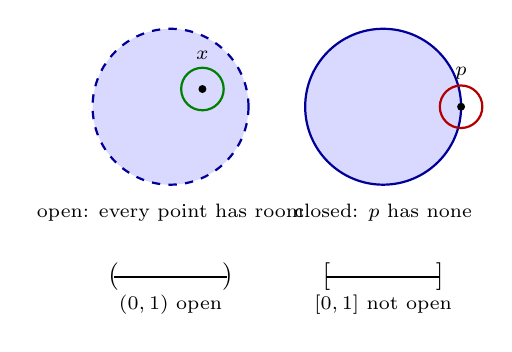
\begin{tikzpicture}[scale=0.9]
                    \fill[blue!15] (0,0) circle (1.1);
                    \draw[blue!60!black,dashed,thick] (0,0) circle (1.1);
                    \fill (0.45,0.25) circle (1.6pt);
                    \node at (0.45,0.72) {\scriptsize $x$};
                    \draw[green!50!black,thick] (0.45,0.25) circle (0.3);
                    \node at (0,-1.5) {\scriptsize open: every point has room};
                    \begin{scope}[shift={(3.0,0)}]
                        \fill[blue!15] (0,0) circle (1.1);
                        \draw[blue!60!black,thick] (0,0) circle (1.1);
                        \fill (1.1,0) circle (1.6pt);
                        \node at (1.1,0.47) {\scriptsize $p$};
                        \draw[red!70!black,thick] (1.1,0) circle (0.3);
                        \node at (0,-1.5) {\scriptsize closed: $p$ has none};
                    \end{scope}
                    \begin{scope}[shift={(0,-2.4)}]
                        \draw[thick] (-0.8,0) -- (0.8,0);
                        \node at (-0.8,0) {$($}; \node at (0.8,0) {$)$};
                        \node at (0,-0.4) {\scriptsize $(0,1)$ open};
                        \draw[thick] (2.2,0) -- (3.8,0);
                        \node at (2.2,0) {$[$}; \node at (3.8,0) {$]$};
                        \node at (3,-0.4) {\scriptsize $[0,1]$ not open};
                    \end{scope}
                \end{tikzpicture}
            \end{column}
            \begin{column}{0.54\textwidth}
                \small
                \textbf{Intuition.} A set is open when \HL{no point of it sits on its
                edge}: from every point you can move a little, in every direction, and
                still be inside. In $[0,1]$ the point $0$ has no such room.

                \vspace{0.3em}
                \textbf{Why these axioms.}
                \begin{itemize}
                    \item \emph{Any union:} each point keeps the room it had in its own set.
                    \item \emph{Finite intersection:} take the smallest of finitely many
                    rooms --- still positive.
                    \item \emph{Not infinite intersection:}
                    $\bigcap_{n\ge1}\bigl(-\tfrac1n,\tfrac1n\bigr)=\{0\}$. The rooms shrink
                    to nothing, and a single point is not open in $\R$.
                \end{itemize}

                \alert{A topology says which points are \emph{near} which, with no numbers
                attached.} The metric on the next slide adds the numbers.
            \end{column}
        \end{columns}
    \end{frame}

    \begin{frame}[shrink=5]{Examples of topologies}
        \small
        \begin{itemize}
            \item \textbf{The usual one on $\R^n$.} Open sets are unions of open balls:
            open intervals on the line, open disks in the plane. Every metric does this
            --- see the next slide.
            \item \textbf{Discrete:} $\Tau_X=2^X$, every subset is open. Every point is
            its own neighbourhood, so nothing is near anything else. \alert{This is what a
            finite point cloud gets from any metric} --- balls small enough to hold one
            point each are open --- which is why we will need a scale $\varepsilon$.
            \item \textbf{Indiscrete:} $\Tau_X=\{\emptyset, X\}$. The opposite extreme:
            no two points can be told apart.
            \item \textbf{A finite one by hand.} On $X=\{a,b,c\}$:
            \[
                \Tau_X=\bigl\{\emptyset,\ \{a\},\ \{a,b\},\ X\bigr\}
                \quad\text{is a topology;}\qquad
                \bigl\{\emptyset,\ \{a\},\ \{b\},\ X\bigr\}\quad\text{is not.}
            \]
            The second fails the union axiom: $\{a\}\cup\{b\}=\{a,b\}$ is missing.
        \end{itemize}

        \vspace{0.3em}
        \begin{alertblock}{What topology keeps, and what it forgets}
            Two spaces are the same topologically (\emph{homeomorphic}) if one can be
            stretched and bent into the other without tearing or gluing. A coffee mug and
            a doughnut are the same; a sphere and a doughnut are not. Topology forgets
            lengths and angles and keeps connectedness and holes --- exactly what the
            Betti numbers count.
        \end{alertblock}
    \end{frame}

    \begin{frame}{Homeomorphism}

        \begin{block}{Continuity}
            A map $f: X\to Y$ is continuous if for every open set $V$ in $Y$, preimage $f^{-1}(V)$ is open in $X$.
        \end{block}

        \begin{block}{Homeomorphism}
            A map $f: X\to Y$ is a homeomorphism if it is continuous and there exists continuous map $g: Y\to X$ such that
            \[(f\circ g) (y) = y \quad \text{ and } \quad (g\circ f)(x)=x\]
            for all $y\in Y$ and all $x\in X$.

            Meaning $g$ and $f$ are inverses of each other.

            If there exists a homeomorphism $f: X\to Y$, then we say that $X$ is homeomorphic to $Y$ (or isomorphic in category of topological spaces).
        \end{block}

    \end{frame}

    \begin{frame}[shrink=3]{Continuity: examples}
        \begin{columns}[T,onlytextwidth]
            \begin{column}{0.56\textwidth}
                \small
                \textbf{$f(x)=x^2$ is continuous.} It is enough to check open intervals
                $V=(a,b)$, since every open set of $\R$ is a union of them:
                \[
                    f^{-1}\bigl((a,b)\bigr)=
                    \begin{cases}
                        \emptyset & b\le 0,\\
                        (-\sqrt b,\ \sqrt b) & a<0<b,\\
                        (-\sqrt b,-\sqrt a)\cup(\sqrt a,\ \sqrt b) & 0\le a.
                    \end{cases}
                \]
                Open in every case. \checkmark

                \vspace{0.4em}
                \textbf{Also continuous:} linear maps, ReLU, $\tanh$, softmax, and any
                composition of them --- so \HL{a neural network with continuous
                activations is a continuous map}.

                \vspace{0.4em}
                \textbf{Intuition.} For metric spaces this is the familiar
                $\varepsilon$--$\delta$ definition: nearby inputs go to nearby outputs.
                A continuous map may stretch, squash or fold; it may not \emph{tear}.
            \end{column}
            \begin{column}{0.42\textwidth}
                \centering
                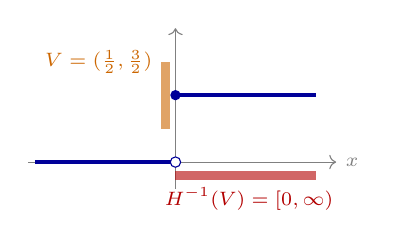
\begin{tikzpicture}[scale=0.85]
                    \draw[->,gray] (-2.2,0) -- (2.4,0) node[right] {\scriptsize $x$};
                    \draw[->,gray] (0,-0.4) -- (0,2.0);
                    \draw[very thick,blue!60!black] (-2.1,0) -- (0,0);
                    \draw[very thick,blue!60!black] (0,1) -- (2.1,1);
                    \fill[blue!60!black] (0,1) circle (2.2pt);
                    \draw[blue!60!black,fill=white] (0,0) circle (2.2pt);
                    \draw[orange!80!black,line width=3pt,opacity=0.6] (-0.15,0.5) -- (-0.15,1.5);
                    \node[orange!80!black,left] at (-0.2,1.5) {\scriptsize $V=(\tfrac12,\tfrac32)$};
                    \draw[red!70!black,line width=3pt,opacity=0.6] (0,-0.2) -- (2.1,-0.2);
                    \node[red!70!black] at (1.1,-0.55) {\scriptsize $H^{-1}(V)=[0,\infty)$};
                \end{tikzpicture}

                \vspace{0.3em}
                \footnotesize\raggedright
                \textbf{Not continuous:} the step $H(x)=1$ for $x\ge0$, $0$ otherwise.
                $V$ is open, but its preimage $[0,\infty)$ is not --- $0$ sits on its edge.
                The jump is the tear.

                \vspace{0.3em}
                The predicted \emph{label} of a classifier, $\arg\max$ of the logits, is a
                step like this: decision boundaries are exactly where continuity fails.
            \end{column}
        \end{columns}
    \end{frame}

    \begin{frame}{Homeomorphisms: examples}
        \begin{columns}[T,onlytextwidth]
            \begin{column}{0.56\textwidth}
                \small
                \textbf{Homeomorphic} --- the same space, topologically:
                \begin{itemize}
                    \item $(-1,1)\cong\R$, by $\tanh:\R\to(-1,1)$ and its inverse
                    $\operatorname{artanh}$. Length is not topological: a short interval and
                    the whole line are the same.
                    \item A circle $\cong$ the boundary of a square, by pushing each point
                    radially outwards (picture). Corners are not topological.
                    \item A coffee mug $\cong$ a doughnut (next slide).
                \end{itemize}

                \vspace{0.4em}
                \textbf{Why $g$ must be continuous too.} $t\mapsto(\cos t,\sin t)$ maps
                $[0,2\pi)$ onto the circle one-to-one and continuously, but it is
                \emph{not} a homeomorphism: points just below $(1,0)$ on the circle come
                from $t\approx2\pi$, points just above it from $t\approx0$. The inverse
                tears the circle open at $(1,0)$.
            \end{column}
            \begin{column}{0.42\textwidth}
                \centering
                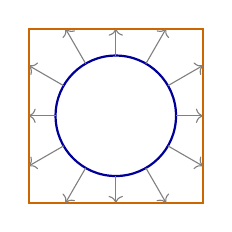
\begin{tikzpicture}[scale=0.85]
                    \draw[thick,blue!60!black] (0,0) circle (0.9);
                    \draw[thick,orange!80!black] (-1.3,-1.3) rectangle (1.3,1.3);
                    \foreach \a in {0,30,...,330}{
                        \draw[->,gray,thin] (\a:0.9) -- ({\a}:{1.3/max(abs(cos(\a)),abs(sin(\a)))});
                    }
                \end{tikzpicture}

                \vspace{0.4em}
                \footnotesize\raggedright
                \textbf{Not homeomorphic:} a line and a circle. Remove one point: the line
                falls into two pieces, the circle stays in one.

                \vspace{0.3em}
                \alert{Homeomorphic spaces have the same Betti numbers}, so different
                Betti numbers \emph{prove} two spaces are different.

                \vspace{0.3em}
                \textbf{In ML:} a normalizing flow is a homeomorphism. A flow from a
                Gaussian blob ($\beta_1=0$) can never produce an exact ring ($\beta_1=1$),
                only approximate one.
            \end{column}
        \end{columns}
    \end{frame}

\newcommand{\clayring}[3]{%
    \draw[blue!60!black,very thick] #1 circle (#2) #1 circle (#3);}
\newcommand{\clayringfill}[3]{%
    \fill[blue!25,even odd rule] #1 circle (#2) #1 circle (#3);}
    \begin{frame}{A coffee mug is a doughnut}
        \begin{center}
            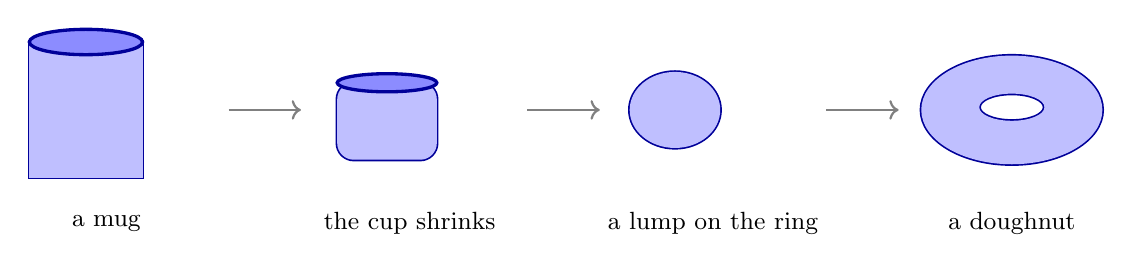
\begin{tikzpicture}[scale=1.15]
                \begin{scope}
                    \clayring{(0.85,0.05)}{0.48}{0.24}
                    \draw[blue!60!black,very thick] (-0.65,-0.75) rectangle (0.6,0.75);
                    \clayringfill{(0.85,0.05)}{0.48}{0.24}
                    \fill[blue!25] (-0.65,-0.75) rectangle (0.6,0.75);
                    \draw[blue!60!black,very thick,fill=blue!45] (-0.025,0.75) ellipse (0.625 and 0.14);
                    \node at (0.2,-1.25) {\small a mug};
                \end{scope}
                \draw[->,thick,gray] (1.55,0) -- (2.35,0);
                \begin{scope}[shift={(3.55,0)}]
                    \clayring{(0.6,0)}{0.52}{0.25}
                    \draw[blue!60!black,very thick,rounded corners=6pt] (-0.8,-0.55) rectangle (0.3,0.3);
                    \clayringfill{(0.6,0)}{0.52}{0.25}
                    \fill[blue!25,rounded corners=6pt] (-0.8,-0.55) rectangle (0.3,0.3);
                    \draw[blue!60!black,very thick,fill=blue!45] (-0.25,0.3) ellipse (0.55 and 0.1);
                    \node at (0,-1.25) {\small the cup shrinks};
                \end{scope}
                \draw[->,thick,gray] (4.85,0) -- (5.65,0);
                \begin{scope}[shift={(6.9,0)}]
                    \draw[blue!60!black,very thick] (-0.42,0) ellipse (0.5 and 0.42);
                    \clayring{(0.4,0)}{0.6}{0.26}
                    \fill[blue!25] (-0.42,0) ellipse (0.5 and 0.42);
                    \clayringfill{(0.4,0)}{0.6}{0.26}
                    \node at (0,-1.25) {\small a lump on the ring};
                \end{scope}
                \draw[->,thick,gray] (8.15,0) -- (8.95,0);
                \begin{scope}[shift={(10.2,0)}]
                    \draw[blue!60!black,very thick] (0,0) ellipse (1.0 and 0.6) (0,0.03) ellipse (0.36 and 0.15);
                    \fill[blue!25,even odd rule] (0,0) ellipse (1.0 and 0.6) (0,0.03) ellipse (0.36 and 0.15);
                    \node at (0,-1.25) {\small a doughnut};
                \end{scope}
            \end{tikzpicture}
        \end{center}

        \vspace{0.8em}
        \small
        Each step only stretches and squashes the clay --- nothing is torn, nothing is
        glued --- so each arrow is a homeomorphism, and so is their composite. The cup's
        hollow was never a hole in the topological sense: it is a dent, and dents flatten
        out. The handle's hole is a hole, and it survives every step.

        \vspace{0.6em}
        \begin{center}
            \alert{All four shapes have $\beta_0=1$, $\beta_1=1$, $\beta_2=0$}: one piece,
            one loop through the handle, no enclosed void.
        \end{center}
    \end{frame}

    \begin{frame}[shrink=3]{Connected spaces}
        \begin{columns}[T,onlytextwidth]
            \begin{column}{0.56\textwidth}
                \small
                \begin{block}{Connected}
                    $X$ is \emph{connected} if it cannot be split as $X=U\cup V$ with $U,V$
                    open, disjoint and both non-empty.
                    It is \emph{path-connected} if any two points are joined by a
                    continuous path $\gamma:[0,1]\to X$.
                \end{block}
                \textbf{Intuition:} one piece. You cannot cut it in two without one of the
                halves having an edge.

                \vspace{0.3em}
                \textbf{Connected:} any interval, $\R^n$, a disk, a circle, a sphere, a
                torus, the mug.

                \vspace{0.2em}
                \textbf{Not connected:} $(0,1)\cup(2,3)$; $\ \R\setminus\{0\}$; two
                clusters; any finite set with more than one point.

                \vspace{0.3em}
                \textbf{Why it matters:} continuous images of connected spaces are
                connected (on $\R$: the intermediate value theorem), and connectedness is
                a homeomorphism invariant --- the ``remove a point'' proof that a line is
                not a circle.
            \end{column}
            \begin{column}{0.42\textwidth}
                \centering
                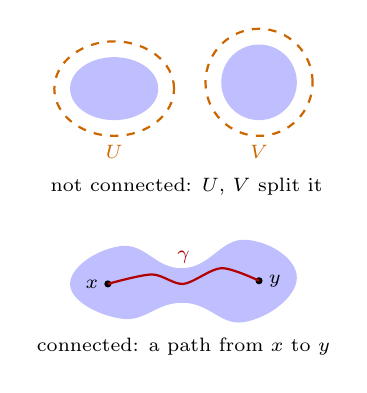
\begin{tikzpicture}[scale=0.8]
                    \fill[blue!25] (-1.1,0) ellipse (0.7 and 0.5);
                    \fill[blue!25] (1.2,0.1) ellipse (0.6 and 0.6);
                    \draw[orange!80!black,dashed,thick] (-1.1,0) ellipse (0.95 and 0.75);
                    \draw[orange!80!black,dashed,thick] (1.2,0.1) ellipse (0.85 and 0.85);
                    \node[orange!80!black] at (-1.1,-1.0) {\scriptsize $U$};
                    \node[orange!80!black] at (1.2,-1.0) {\scriptsize $V$};
                    \node at (0.05,-1.55) {\scriptsize not connected: $U$, $V$ split it};
                    \begin{scope}[shift={(0,-3.1)}]
                        \fill[blue!25] plot[smooth cycle,tension=0.8]
                            coordinates {(-1.8,0) (-1.0,0.6) (0,0.25) (1.0,0.7) (1.8,0.1) (1.0,-0.6) (0,-0.3) (-1.0,-0.55)};
                        \fill (-1.2,0) circle (1.6pt) node[left] {\scriptsize $x$};
                        \fill (1.2,0.05) circle (1.6pt) node[right] {\scriptsize $y$};
                        \draw[red!70!black,thick] plot[smooth] coordinates {(-1.2,0) (-0.5,0.15) (0,0) (0.6,0.25) (1.2,0.05)};
                        \node[red!70!black] at (0,0.42) {\scriptsize $\gamma$};
                        \node at (0,-1.0) {\scriptsize connected: a path from $x$ to $y$};
                    \end{scope}
                \end{tikzpicture}

                \vspace{0.4em}
                \footnotesize\raggedright
                \alert{$\beta_0$ counts connected components.} Clustering is finding
                them, and tracking components across scales (persistence in dimension
                $0$) turns out to be single-linkage clustering (Part 4).
            \end{column}
        \end{columns}
    \end{frame}

    \begin{frame}[shrink=3]{Compact spaces}
        \begin{columns}[T,onlytextwidth]
            \begin{column}{0.56\textwidth}
                \small
                \begin{block}{Compact}
                    $X$ is \emph{compact} if every cover of $X$ by open sets has a finite
                    subcover: whenever $X=\bigcup_{i\in I}U_i$ with each $U_i$ open, already
                    $X=U_{i_1}\cup\dots\cup U_{i_n}$ for finitely many of them.
                \end{block}
                \textbf{Intuition:} nothing escapes to infinity and nothing leaks out
                through a missing edge. In $\R^n$, compact $=$ \HL{closed and bounded}
                (Heine--Borel).

                \vspace{0.3em}
                \textbf{Compact:} $[0,1]$, a closed disk, a circle, a sphere, a torus,
                \emph{every finite set} --- so every point cloud.

                \vspace{0.2em}
                \textbf{Not compact:} $\R$, covered by $(-n,n)$; $\ (0,1)$, covered by
                $(\tfrac1n,1)$ (picture); an open disk.

                \vspace{0.3em}
                \textbf{Why it matters:} a continuous $f:X\to\R$ on a compact $X$ attains
                its max and min --- why a loss on a compact parameter set has a
                minimiser. Continuous images of compact spaces are compact.
            \end{column}
            \begin{column}{0.42\textwidth}
                \centering
                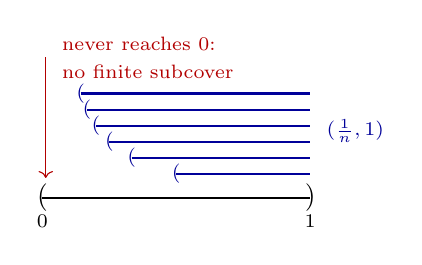
\begin{tikzpicture}[scale=0.85]
                    \draw[thick] (0,0) -- (4,0);
                    \node at (0,0) {$($}; \node at (4,0) {$)$};
                    \node at (0,-0.35) {\scriptsize $0$}; \node at (4,-0.35) {\scriptsize $1$};
                    \foreach \n in {2,...,7}{
                        \draw[blue!60!black,thick] ({4/\n},{0.12+0.24*(\n-1)}) -- (4,{0.12+0.24*(\n-1)});
                        \node[blue!60!black] at ({4/\n},{0.12+0.24*(\n-1)}) {\scriptsize $($};
                    }
                    \node[blue!60!black,right] at (4.1,1.0) {\scriptsize $(\tfrac1n,1)$};
                    \draw[->,red!70!black] (0.05,2.1) -- (0.05,0.3);
                    \node[red!70!black,align=left,right] at (0.15,2.1) {\scriptsize never reaches $0$:\\[-2pt] \scriptsize no finite subcover};
                \end{tikzpicture}

                \vspace{0.3em}
                \footnotesize\raggedright
                Each interval misses a little near $0$, and finitely many of them miss
                the part below the smallest $\tfrac1n$. In $[0,1]$ the point $0$ is
                present, and any open set covering it reaches some $\tfrac1n$: then
                finitely many suffice.

                \vspace{0.3em}
                \alert{For TDA:} a compact space can be covered by finitely many
                $\varepsilon$-balls for every $\varepsilon>0$ --- so a finite sample can
                approximate it at every resolution.
            \end{column}
        \end{columns}
    \end{frame}

    \begin{frame}[shrink=8]{Metric space}
        \begin{block}{Metric Space}
            A metric space is a pair $(X, d)$, where $X$ is a set of points, and $d: X\times X\to \mathbb{R}^{\geq 0}$ is a distance function subject to the following axioms:
            \begin{enumerate}
                \item $d(x,y)=0 \iff x=y$,
                \item Symmetry $d(x,y)=d(y,x)$,
                \item The triangle inequality: $d(x,z)\le d(x,y)+d(y,z)$.
            \end{enumerate}
        \end{block}

        The distance can be Euclidean on a raw feature vector, cosine or correlation distance on an embedding, a learned metric, edit distance on strings, or a graph shortest path.

        \begin{block}{Open balls}
            An open ball $B(x, \varepsilon)$ is a set of all points $y$ that are closer than the distance $\varepsilon$, meaning $B(x,\varepsilon)=\{y: d(x,y)<\varepsilon \}$.
        \end{block}

        \vspace{0.5em}
        \alert{The open balls of the metric generate a topology on $X$.}
    \end{frame}

    \begin{frame}[shrink=10]{Hausdorff distance: how far apart two point clouds are}
        \begin{block}{Hausdorff distance}
            For finite $X,Y$ in a metric space,
            \[
                \dH(X,Y)\;=\;\max\Bigl\{\ \max_{x\in X}\ \min_{y\in Y} d(x,y),\ \
                \max_{y\in Y}\ \min_{x\in X} d(x,y)\ \Bigr\}.
            \]
            Equivalently: the smallest $r$ such that every point of $X$ is within $r$ of
            some point of $Y$, \emph{and} every point of $Y$ is within $r$ of some point
            of $X$.
        \end{block}
        \begin{columns}[T,onlytextwidth]
            \begin{column}{0.52\textwidth}
                \centering
                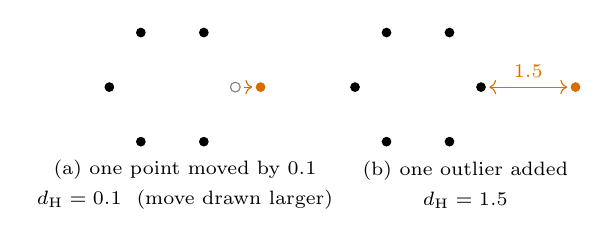
\begin{tikzpicture}[scale=0.8]
                    \foreach \a in {60,120,180,240,300}{\fill (\a:1) circle (2.2pt);}
                    \draw[gray] (0:1) circle (2.2pt);
                    \fill[orange!85!black] (0:1.4) circle (2.2pt);
                    \draw[->,orange!85!black,shorten <=3pt,shorten >=3pt] (0:1) -- (0:1.4);
                    \node[align=center] at (0.2,-1.55)
                        {\scriptsize (a) one point moved by $0.1$\\[-1pt]
                         \scriptsize $\dH=0.1$ \ (move drawn larger)};
                    \begin{scope}[shift={(3.9,0)}]
                        \foreach \a in {0,60,...,300}{\fill (\a:1) circle (2.2pt);}
                        \fill[orange!85!black] (2.5,0) circle (2.2pt);
                        \draw[<->,orange!85!black,shorten <=3pt,shorten >=3pt] (1,0) -- (2.5,0)
                            node[midway,above] {\scriptsize $1.5$};
                        \node[align=center] at (0.75,-1.55)
                            {\scriptsize (b) one outlier added\\[-1pt] \scriptsize $\dH=1.5$};
                    \end{scope}
                \end{tikzpicture}
            \end{column}
            \begin{column}{0.46\textwidth}
                \small
                \textbf{Computing it.} Form the $|X|\times|Y|$ distance matrix. Take each
                row's minimum and the largest of those; the same for columns; then the
                larger of the two.

                \vspace{0.3em}
                \textbf{Both directions matter.} In (b) every point of $X$ is in $Y$, so
                the first term is $0$; the outlier alone makes the second term $1.5$.

                \vspace{0.3em}
                Part 4 uses $\dH$ to measure how much the \emph{data} moved.
            \end{column}
        \end{columns}
    \end{frame}

    \begin{frame}{Thicken the points}
        \textbf{The problem.} A finite point cloud is topologically trivial: $n$ isolated
        points, $\beta_0=n$.
        The loop from data set (b) is not \emph{in} the points --- it is in how they sit relative to each other at a certain \emph{scale}.

        \vspace{0.5em}
        So: introduce a scale, and build something with actual shape.\par
        \vspace{0.3em}
        \small
        Fix $\varepsilon>0$ and replace each point by a ball of radius $\varepsilon/2$.
        Let's consider the union $\bigcup_i B(x_i,\varepsilon/2)$.
        \begin{center}
            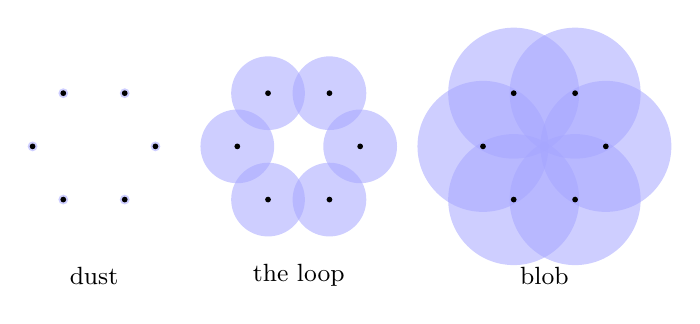
\begin{tikzpicture}[scale=0.52]
\foreach \s/\rad/\lab in {0/0.12/{\small dust}, 5.0/0.9/{\small \alert{the loop}}, 11.0/1.6/{\small blob}} {
    \begin{scope}[shift={(\s,0)}]
        \hexpoints
        \foreach \i in {1,...,6}{\fill[blue!35,opacity=0.55] (P\i) circle (\rad);}
        \hexdots
        \node at (0,-3.15) {\lab};
    \end{scope}}
            \end{tikzpicture}
        \end{center}
        \vspace{-0.3em}
    \end{frame}

    \begin{frame}{Simplicial complexes, in one slide}
        \small
        A \HL{$k$-simplex} is a set of $k+1$ vertices: a point, an edge, a triangle, a
        tetrahedron. Think of it as the convex hull, but store it as the set.
        \begin{center}
            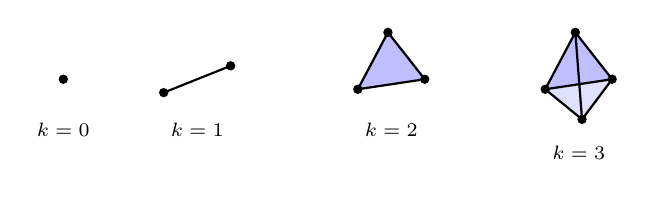
\begin{tikzpicture}[scale=0.85]
  \fill (0,0) circle (2pt); \node[font=\scriptsize] at (0,-0.75) {$k=0$};
  \begin{scope}[shift={(2.0,0)}]
      \draw[thick] (-0.5,-0.2)--(0.5,0.2); \fill (-0.5,-0.2) circle (2pt); \fill (0.5,0.2) circle (2pt);
      \node[font=\scriptsize] at (0,-0.75) {$k=1$};
  \end{scope}
  \begin{scope}[shift={(4.4,-0.15)}]
      \fill[blue!25] (0,0)--(1,0.15)--(0.45,0.85)--cycle;
      \draw[thick] (0,0)--(1,0.15)--(0.45,0.85)--cycle;
      \foreach \p in {(0,0),(1,0.15),(0.45,0.85)}{\fill \p circle (2pt);}
      \node[font=\scriptsize] at (0.5,-0.6) {$k=2$};
  \end{scope}
  \begin{scope}[shift={(7.2,-0.15)}]
      \fill[blue!25] (0,0)--(1,0.15)--(0.45,0.85)--cycle;
      \fill[blue!12] (0,0)--(1,0.15)--(0.55,-0.45)--cycle;
      \draw[thick] (0,0)--(1,0.15)--(0.45,0.85)--cycle;
      \draw[thick] (0,0)--(0.55,-0.45)--(1,0.15); \draw[thick] (0.55,-0.45)--(0.45,0.85);
      \foreach \p in {(0,0),(1,0.15),(0.45,0.85),(0.55,-0.45)}{\fill \p circle (2pt);}
      \node[font=\scriptsize] at (0.5,-0.95) {$k=3$};
  \end{scope}
            \end{tikzpicture}
        \end{center}
        \begin{block}{Simplicial complex}
            A collection $K$ of finite nonempty vertex sets, closed under taking subsets:
            if $\sigma\in K$ and $\emptyset\neq\tau\subseteq\sigma$ then $\tau\in K$.
        \end{block}
        \emph{``If the triangle is in, so are its three edges and three vertices.''}
        That is the whole definition: a list of subsets, so a computer can hold it exactly
        the way it already holds a sparse graph.
    \end{frame}

    \begin{frame}[shrink=5]{The Vietoris--Rips complex}
        \begin{block}{Definition}
            \[
                \VR_\varepsilon(X)\;=\;\bigl\{\ \sigma\subseteq X \ :\ d(x,y)\le\varepsilon
                \ \text{ for all } x,y\in\sigma\ \bigr\}.
            \]
        \end{block}
        Build the graph on $X$ with an edge whenever $d(x,y)\le\varepsilon$ --- exactly your
        usual $\varepsilon$-neighbourhood graph --- then fill in \emph{every} clique.
        Nothing but the distance matrix is used.

        \vspace{0.6em}
        \begin{center}
            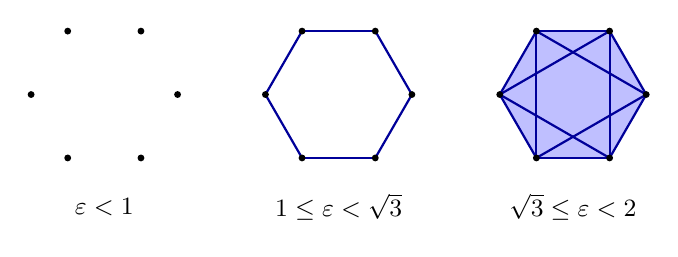
\begin{tikzpicture}[scale=0.62]
\begin{scope}
    \hexpoints \hexdots \node at (0,-2.3) {\small $\varepsilon<1$};
\end{scope}
\begin{scope}[shift={(4.8,0)}]
    \hexpoints
    \foreach \i/\j in {1/2,2/3,3/4,4/5,5/6,6/1}{\draw[thick,blue!60!black] (P\i)--(P\j);}
    \hexdots \node at (0,-2.3) {\small $1\le\varepsilon<\sqrt3$};
\end{scope}
\begin{scope}[shift={(9.6,0)}]
    \hexpoints
    \foreach \i/\j/\k in {1/2/3,3/4/5,5/6/1,1/3/5}{\fill[blue!25] (P\i)--(P\j)--(P\k)--cycle;}
    \foreach \i/\j in {1/2,2/3,3/4,4/5,5/6,6/1,1/3,3/5,5/1,2/4,4/6,6/2}{\draw[thick,blue!60!black] (P\i)--(P\j);}
    \hexdots \node at (0,-2.3) {\small $\sqrt3\le\varepsilon<2$};
\end{scope}
            \end{tikzpicture}
        \end{center}
        \vspace{-0.2em}
        \small Six points on the unit circle. At $\varepsilon=1$ the hexagon closes: the loop
        appears. At $\varepsilon=\sqrt3$ the triangles fill in and it is gone.
    \end{frame}

    \ifcomputedslides
    \begin{frame}{The Vietoris--Rips complex, as $\varepsilon$ grows}
        \begin{center}
            \IfFileExists{output/rips_hexagon_frames/frame-000.png}
            {\animategraphics[width=\textwidth,height=0.52\textheight,keepaspectratio,
                controls,loop,autoplay,poster=50]{15}{output/rips_hexagon_frames/frame-}{000}{089}}
            {\figmissing{rips_hexagon_frames/frame-000}}
        \end{center}
        \vspace{-0.3em}
        {\footnotesize The three pictures from the previous slide, as one sweep of
            $\varepsilon$ from $0$ to $2.2$. Right: the barcode, one bar per feature ---
            the $H_0$ row tracks components, the $H_1$ row loops. The bars under the
            moving line are the features alive at that scale: count them to get
            $\beta_0$ and $\beta_1$ of the complex on the left.\par}
        \vspace{0.2em}
        \figcredit{rips\_animation.py}
    \end{frame}
    \fi

    \ifcomputedslides
    \begin{frame}{The same six points, actually computed}
        \computedfigside[0.60]{talk_02_complexes}{%
            \textbf{Top:} the Rips complex in each regime, with its simplex counts and
            Betti numbers underneath. \textbf{Bottom:} the union of balls it stands in
            for. At $\varepsilon=\sqrt3$ Rips has $6$ vertices, $12$ edges and $8$
            triangles --- the boundary of an octahedron ---
            \alert{but the balls plainly still miss the centre}. The hole is real; Rips
            filled it in anyway.}{talk\_02\_complexes.py}
    \end{frame}
    \fi

    \begin{frame}{Two better (and pricier) alternatives}
        \small
        \begin{block}{\v{C}ech complex}
            $\sigma\in\Cechsym_\varepsilon(X)$ iff the balls $B(x,\varepsilon/2)$, $x\in\sigma$,
            share a common point. It has \emph{exactly} the topology of the union of balls
            (the nerve theorem). Expensive: you must test intersections, not just pairwise
            distances.
        \end{block}
        \begin{block}{Alpha complex}
            Intersect the balls with their Voronoi cells first. Same guarantee as \v{C}ech, but
            only $O(n^{\lceil d/2\rceil})$ simplices --- cheap in low-dimensional Euclidean data,
            useless once $d$ is the size of an embedding.
        \end{block}
        \vspace{0.3em}

        \begin{center}
            \alert{Rips is the default in high dimension because it needs nothing but the
            distance matrix} --- the same reason $k$-NN graphs are cheap and Voronoi diagrams
            are not.
        \end{center}
        \vspace{0.2em}
        {\scriptsize On those same six points, \texttt{talk\_02\_complexes.py} builds
        both: at $\varepsilon=\sqrt3$ Rips gives $\beta_1=0$ and \v{C}ech still gives
            $\beta_1=1$. \v{C}ech is right --- and it needed the coordinates and a
        smallest-enclosing-ball test to be so.\par}
    \end{frame}

    \begin{frame}{The problem we are not going to solve yet}
        \begin{center}
            \Large \alert{Which $\varepsilon$?}
        \end{center}

        \vspace{0.5em}
        \begin{itemize}
            \item $\varepsilon$ too small: $\VR_\varepsilon(X)$ is $n$ isolated points. \emph{Dust.}
            \item $\varepsilon$ too large: $\VR_\varepsilon(X)$ is one giant simplex,
            contractible. \emph{Blob.}
            \item In between: the loop. But the window depends on the sampling density,
            which you do not know.
        \end{itemize}

        \vspace{0.7em}

        There is no principled choice, and any single choice is fragile: one outlier moves it
        --- the same fragility that makes a single choice of $k$ or $\varepsilon$ for a
        neighbourhood graph feel arbitrary.

        \vspace{0.7em}
        \begin{alertblock}{Hold this thought}
            We come back in Part 4 with an answer that avoids choosing:
            \HL{compute at every $\varepsilon$ at once and record how long each feature lasts.}
            First we need to know how to count holes at a \emph{fixed} $\varepsilon$.
        \end{alertblock}
    \end{frame}

    \section{Homology}

    \begin{frame}[shrink=5]{You already know a special case}
        Recall the graph Laplacian $L=D-A$ (degree minus adjacency), or equivalently
        $L=BB^{\mathsf T}$ for the signed incidence matrix $B$. Spectral clustering
        \emph{(von Luxburg 2007)} and graph convolutional networks
        \emph{(Kipf \& Welling 2017)} both lean on one basic fact:
        \[
            \dim\ker L \;=\; \text{number of connected components of the graph.}
        \]
        You have almost certainly used this without calling it a Betti number.

        \vspace{0.7em}
        \begin{alertblock}{The whole talk, in one promise}
            \begin{enumerate}
                \item Replace \emph{graph} by \emph{simplicial complex} --- cliques and triangles,
                not just edges.
                \item Replace \emph{connected components} ($k=0$) by \emph{$k$-dimensional holes}
                --- loops, voids, and beyond.
            \end{enumerate}
            The same fact --- kernel dimension counts topological features --- holds at every
            level $k$, for a matrix $L_k$ that specialises to your familiar graph Laplacian at
            $k=0$. Parts 3--5 build the machinery; \HL{Part 6 delivers $L_k$ and proves it.}
        \end{alertblock}
    \end{frame}

    \begin{frame}{Chains are vectors}
        Let $n_k$ be the number of $k$-simplices of $K$.

        \begin{block}{Chain space}
            $C_k = \R^{n_k}$, with one coordinate per $k$-simplex.
        \end{block}

        So $C_0=\R^{\#\text{vertices}}$, $C_1=\R^{\#\text{edges}}$, $C_2=\R^{\#\text{triangles}}$.
        A \HL{$k$-chain} is a formal weighted sum of $k$-simplices --- for $k=1$, think of a
        weighted set of edges, like a flow on a network.

        \vspace{0.7em}
        \begin{block}{Orientation: the entire convention}
            Fix once and for all a total order on the vertices, and always write a simplex with
            its vertices increasing: $[v_0<v_1<\dots<v_k]$. That is it.
        \end{block}
        Signs will appear below. They are bookkeeping so that ``going around a loop
        one way'' is the negative of ``going the other way''.
        \HL{Over $\bF_2$ all signs are $1$ and you can ignore this slide entirely.}
    \end{frame}

    \begin{frame}[shrink=12]{The boundary operator is a matrix}
        \begin{block}{Definition}
            $\partial_k : C_k\to C_{k-1}$ is the linear map defined on basis vectors by
            \[
                \partial_k\,[v_0,\dots,v_k]\;=\;\sum_{i=0}^{k}\,(-1)^i\,[v_0,\dots,\widehat{v_i},\dots,v_k],
            \]
            where $\widehat{v_i}$ means ``delete $v_i$''.
        \end{block}

        \vspace{0.4em}
        Concretely, for the cases we care about:
        \[
            \partial_1[a,b] = b-a, \qquad
            \partial_2[a,b,c] = [b,c]-[a,c]+[a,b].
        \]

        \vspace{0.4em}

        \textbf{As a matrix.} $\partial_k$ is $n_{k-1}\times n_k$; the column of $\sigma$ has a
        $\pm1$ in the row of each face of $\sigma$ and $0$ elsewhere. Very sparse: each
        column has exactly $k+1$ nonzeros.

        \vspace{0.4em}
        For $k=1$ this \emph{is} the signed incidence matrix $B$ from the previous slide.
        $\partial_1$ is not a new object --- it is the one you already had a name for.
    \end{frame}

    \begin{frame}{Our running example}
        \begin{columns}[T,onlytextwidth]
            \begin{column}{0.36\textwidth}
                \centering
                \spinetriangle{}
            \end{column}
            \begin{column}{0.62\textwidth}
                \small
                Vertices $a<b<c$; edges $e_1=[a,b]$, $e_2=[b,c]$, $e_3=[a,c]$.
                \[
                    \partial_1=
                    \bordermatrix{ & e_1 & e_2 & e_3 \cr
                    a & -1 & 0 & -1 \cr
                    b & 1 & -1 & 0 \cr
                    c & 0 & 1 & 1 \cr}
                \]
                \vspace{-0.3em}
                Read a column: ``$\partial_1 e_1 = b-a$'' --- head minus tail.

                \vspace{0.6em}
                If the triangle $t=[a,b,c]$ is present as well,
                \[
                    \partial_2 t = [b,c]-[a,c]+[a,b] = e_1+e_2-e_3,
                    \qquad
                    \partial_2=\begin{pmatrix}
                                   1\\ 1\\ -1
                    \end{pmatrix}.
                \]
            \end{column}
        \end{columns}
        \vspace{0.5em}

        \begin{center}
            Two matrices. Everything else in this part is what you can read off them.
        \end{center}
    \end{frame}

    \begin{frame}[shrink=8]{$\partial\circ\partial=0$ is a matrix product}
        \begin{block}{The fundamental identity}
            \[
                \partial_k\,\partial_{k+1}\;=\;0.
            \]
        \end{block}

        On our example, just multiply:
        \[
            \partial_1\partial_2=
            \begin{pmatrix}
                -1&0&-1\\ 1&-1&0\\ 0&1&1
            \end{pmatrix}
            \begin{pmatrix}
                1\\ 1\\ -1
            \end{pmatrix}
            =\begin{pmatrix}
                 -1+0+1\\ 1-1+0\\ 0+1-1
            \end{pmatrix}
            =\begin{pmatrix}
                 0\\0\\0
            \end{pmatrix}.
        \]

        \vspace{0.3em}
        \textbf{Why in general.} Deleting two vertices $v_i,v_j$ from $\sigma$ can be done in
        two orders, and the two resulting signs are opposite. Every codimension-$2$ face is
        produced exactly twice and cancels.

        \vspace{0.5em}
        \begin{alertblock}{What it buys us}
            $\partial_k\partial_{k+1}=0$ says exactly
            $\ \im\partial_{k+1}\subseteq\ker\partial_k$: \HL{every boundary is a cycle.}
            So the quotient on the next slide makes sense.
        \end{alertblock}
    \end{frame}

    \begin{frame}[shrink=8]{Cycles, boundaries, Betti numbers}
        \begin{block}{}
            \[
                Z_k=\ker\partial_k \quad\text{(\HL{cycles})},\qquad
                B_k=\im\partial_{k+1}\quad\text{(\HL{boundaries})},\qquad
                H_k = Z_k/B_k .
            \]
        \end{block}

        \vspace{0.3em}
        \begin{itemize}
            \item A \emph{cycle} is a chain with no boundary --- a closed loop, a closed surface.
            \item A cycle is \emph{uninteresting} if it is already the boundary of something one
            dimension up: the rim of a filled triangle is a loop, but it encloses nothing.
            \item $H_k$ = cycles \alert{modulo} those that bound. Its dimension counts genuine
            $k$-dimensional holes.
        \end{itemize}

        \vspace{0.5em}

        \begin{alertblock}{Rank--nullity, and we are done}
            \[
                \beta_k \;=\;\dim Z_k-\dim B_k
                \;=\;\underbrace{\bigl(n_k-\rank\partial_k\bigr)}_{\nullity\partial_k}-\rank\partial_{k+1}.
            \]
        \end{alertblock}
        Computing homology $=$ computing the ranks of two sparse $0,\pm1$ matrices --- the
        same computation your linear-algebra library already does for you.
    \end{frame}

    \begin{frame}{Hollow versus filled}
        \begin{columns}[T,onlytextwidth]
            \begin{column}{0.30\textwidth}
                \centering
                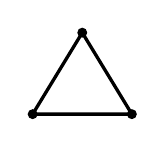
\begin{tikzpicture}[scale=0.9]
  \coordinate (a) at (0,0); \coordinate (b) at (1.4,0); \coordinate (c) at (0.7,1.15);
  \draw[very thick] (a)--(b)--(c)--cycle;
  \foreach \p in {a,b,c}{\fill (\p) circle (2pt);}
                \end{tikzpicture}\\
                {\scriptsize $K$: no triangle}\\[1.0em]
                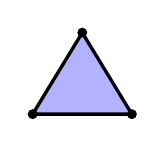
\begin{tikzpicture}[scale=0.9]
  \coordinate (a) at (0,0); \coordinate (b) at (1.4,0); \coordinate (c) at (0.7,1.15);
  \fill[blue!30] (a)--(b)--(c)--cycle;
  \draw[very thick] (a)--(b)--(c)--cycle;
  \foreach \p in {a,b,c}{\fill (\p) circle (2pt);}
                \end{tikzpicture}\\
                {\scriptsize $K'=K\cup\{t\}$}
            \end{column}
            \begin{column}{0.68\textwidth}
                \small
                Row-reduce $\partial_1$: $\rank\partial_1=2$ (the three columns sum to zero, any two
                are independent).

                \vspace{0.4em}
                \textbf{Dimension 0.} $\partial_0=0$, so
                $\beta_0 = n_0-\rank\partial_1 = 3-2 = 1$. \checkmark\ one component.

                \vspace{0.4em}
                \textbf{Dimension 1.} $\ \dim Z_1=n_1-\rank\partial_1=3-2=1$,
                spanned by $z=e_1+e_2-e_3$ --- go $a\to b\to c$, come back along $ac$.

                \vspace{0.5em}

                \emph{Hollow:} no triangles, so $\partial_2=0$, $\rank\partial_2=0$:
                \[ \beta_1 = 1-0 = \boxed{1}. \]

                \emph{Filled:} $\partial_2 t=e_1+e_2-e_3=z$, so $\rank\partial_2=1$:
                \[ \beta_1 = 1-1 = \boxed{0}. \]
                The one cycle now bounds. The hole is gone.
            \end{column}
        \end{columns}
    \end{frame}

    \ifcomputedslides
    \begin{frame}{Hollow versus filled, actually computed}
        \computedfig[0.56]{talk_03_homology}{%
            The computation from the previous slide, done by the code in the same edge order. $\partial_1$ has
            rank $2$, so its kernel is one-dimensional and spanned by $z$, drawn on the left
            as a flow round the triangle. Filling in $t$ adds one column to $\partial_2$, and
            that column \emph{is} $z$: the cycle is now a boundary and $\beta_1$ drops from
            $1$ to $0$.}{talk\_03\_homology.py}
    \end{frame}
    \fi

    \begin{frame}{Boundary of a tetrahedron}
        \small
        $K=$ all proper faces of $[1,2,3,4]$: $4$ vertices, $6$ edges, $4$ triangles,
        \alert{no} solid. Topologically a sphere $S^2$.

        \vspace{0.5em}
        \begin{columns}[T,onlytextwidth]
            \begin{column}{0.30\textwidth}
                \centering
                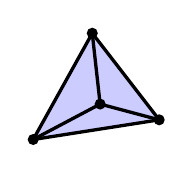
\begin{tikzpicture}[scale=1.0]
  \coordinate (p1) at (0,0); \coordinate (p2) at (1.6,0.25);
  \coordinate (p3) at (0.75,1.35); \coordinate (p4) at (0.85,0.45);
  \fill[blue!20] (p1)--(p2)--(p3)--cycle;
  \draw[very thick] (p1)--(p2)--(p3)--cycle;
  \draw[very thick] (p1)--(p4)--(p2); \draw[very thick] (p4)--(p3);
  \foreach \p in {p1,p2,p3,p4}{\fill (\p) circle (2pt);}
                \end{tikzpicture}
            \end{column}
            \begin{column}{0.66\textwidth}
                Counts: $n_0=4$, $n_1=6$, $n_2=4$.
                \begin{itemize}
                    \item $\rank\partial_1=3$ (connected: $n_0-1$).
                    \item $\rank\partial_2=3$ (the four triangle columns sum to zero, any three
                    are independent).
                    \item $\beta_0=4-3=1$. \checkmark
                    \item $\beta_1=(6-3)-3=0$. \checkmark\ no loops on a sphere
                    \item $\beta_2=(4-3)-0=1$. \checkmark\ one enclosed void
                \end{itemize}
                Euler: $4-6+4=2=1-0+1$. \checkmark
            \end{column}
        \end{columns}

        \vspace{0.5em}

        The single element of $\ker\partial_2$ is the sum of all four triangles with signs ---
        the closed surface itself. \alert{It is a cycle that bounds nothing, because we never
        put in the solid tetrahedron.} Add the solid and $\beta_2$ drops to $0$: this is the
        $k{=}2$ analogue of filling the triangle two slides ago.
    \end{frame}

    \begin{frame}[shrink=8]{Three sanity checks}
        \begin{block}{$\beta_0$ counts connected components}
            For a graph, $\rank\partial_1 = n_0-c$ where $c$ is the number of components. So
            $\beta_0=n_0-\rank\partial_1=c$ --- the same fact from two slides ago, restated. \checkmark
        \end{block}

        \begin{block}{$\beta_1$ of a graph is its cycle rank}
            No triangles $\Rightarrow \partial_2=0 \Rightarrow \beta_1=n_1-\rank\partial_1=E-(V-1)$.
            This is $E-V+1$: the number of edges outside a spanning tree, exactly what
            Kruskal's or Prim's algorithm leaves out.
        \end{block}

        \begin{block}{Euler characteristic}
            $\sum_k(-1)^kn_k=\sum_k(-1)^k\beta_k$, since the ranks cancel in pairs in
            $\beta_k=n_k-\rank\partial_k-\rank\partial_{k+1}$. A cheap and effective debugging tool.
        \end{block}

        \vspace{0.2em}

        \textbf{Reference values.} circle $(1,1,0)$; sphere $S^2$ $(1,0,1)$;
        torus $(1,2,1)$; disk $(1,0,0)$.
    \end{frame}

    \begin{frame}{What it costs, and why the answer is a shape invariant}
        \begin{columns}[T,onlytextwidth]
            \begin{column}{0.49\textwidth}
                \begin{block}{Cost}
                    \scriptsize
                    Two rank computations on sparse $0,\pm1$ matrices --- Gaussian elimination,
                    $O(n_k^2 n_{k-1})$ worst case.

                    \vspace{0.3em}
                    The real cost is \alert{size}: a Rips complex on $n$ points has up to
                    $\binom{n}{k+1}$ $k$-simplices. $n=1000$, $k=2$: $1.7\times 10^8$ triangles.
                    Cap the dimension, cap $\varepsilon$ --- the same trade-off as capping the degree
                    in a $k$-NN graph.
                \end{block}
            \end{column}
            \begin{column}{0.49\textwidth}
                \begin{block}{Invariance}
                    \scriptsize
                    $\beta_k$ depends only on the \emph{shape}, not on the triangulation: two complexes
                    that can be continuously deformed into one another have the same Betti numbers.

                    \vspace{0.3em}
                    We will use this, not prove it. It is the reason $\beta_k$ deserves to be called an
                    invariant of the data rather than an artifact of how we built the complex.
                \end{block}
            \end{column}
        \end{columns}

        \vspace{0.7em}

        \begin{alertblock}{Part 3 in one line}
            \[
                \beta_k=\nullity\partial_k-\rank\partial_{k+1}.
            \]
            \centering Homology is a rank computation.
        \end{alertblock}
    \end{frame}

    \section{4. Persistence}

    \begin{frame}[shrink=5]{Sweep $\varepsilon$ instead of choosing it}
        As $\varepsilon$ grows, simplices are only ever \emph{added}:
        \[
            \varepsilon\le\varepsilon' \;\Longrightarrow\; \VR_\varepsilon(X)\subseteq\VR_{\varepsilon'}(X).
        \]
        This nested family is a \HL{filtration}. Equivalently: order the simplices so that
        every simplex comes after all of its faces, and insert them one at a time --- exactly
        like building a minimum spanning tree by adding edges in increasing weight order.

        \vspace{0.7em}

        Each insertion does exactly one of two things to homology:
        \begin{itemize}
            \item it \HL{creates} a new cycle --- a feature is \alert{born}; or
            \item it \HL{fills in} an existing cycle --- a feature \alert{dies}.
        \end{itemize}

        \vspace{0.5em}
        Record the pair $(\text{birth},\text{death})$ for every feature. That list is the
        answer, and it required no choice of $\varepsilon$.

        \vspace{0.5em}

        \textbf{Elder rule.} When two features merge, the older one survives and the younger
        one dies. This makes the pairing well defined.
    \end{frame}

    \begin{frame}{Barcodes and diagrams}
        \begin{columns}[T,onlytextwidth]
            \begin{column}{0.58\textwidth}
                \small
                \textbf{Which features?} The classes of $H_k=Z_k/B_k$ from Part 3:
                $H_0$ = components, $H_1$ = loops, $H_2$ = voids. An ``$H_k$ bar'' is one
                $k$-dimensional hole, and at any $\varepsilon$ the number of $H_k$ bars
                alive is $\beta_k$.

                \vspace{0.5em}
                \textbf{Barcode}: draw each feature as a horizontal bar from its birth to its death,
                grouped by dimension $k$.

                \vspace{0.5em}
                \textbf{Persistence diagram}: plot each feature as the point
                $(\text{birth},\text{death})$ above the diagonal.

                \vspace{0.5em}
                \textbf{Persistence} $=\ \text{death}-\text{birth}$, the distance from the diagonal.

                \vspace{0.7em}
                \alert{Heuristic:} long bars are features of the underlying shape, short bars are
                sampling noise. The stability slide says why you are allowed to believe this.
            \end{column}
            \begin{column}{0.4\textwidth}
                \centering
                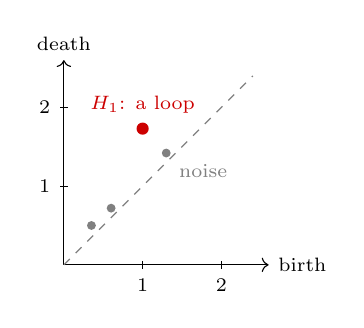
\begin{tikzpicture}[scale=1.0]
  \draw[->] (0,0)--(2.6,0) node[right] {\scriptsize birth};
  \draw[->] (0,0)--(0,2.6) node[above] {\scriptsize death};
  \draw[dashed,gray] (0,0)--(2.4,2.4);
  \fill[red!80!black] (1,1.73) circle (2.2pt);
  \node[red!80!black,above] at (1,1.8) {\scriptsize $H_1$: a loop};
  \fill[gray] (0.6,0.72) circle (1.6pt);
  \fill[gray] (1.3,1.42) circle (1.6pt);
  \fill[gray] (0.35,0.5) circle (1.6pt);
  \node[gray,below right] at (1.34,1.40) {\scriptsize noise};
  \foreach \x in {1,2}{\draw (\x,0.05)--(\x,-0.05) node[below] {\scriptsize \x};}
  \foreach \y in {1,2}{\draw (0.05,\y)--(-0.05,\y) node[left] {\scriptsize \y};}
                \end{tikzpicture}
            \end{column}
        \end{columns}
    \end{frame}

    \begin{frame}[shrink=15]{The hexagon, end to end}
        \begin{columns}[T,onlytextwidth]
            \begin{column}{0.45\textwidth}
                \small
                Six points on the unit circle. Distances: $1$ (adjacent), $\sqrt3$ (short diagonal),
                $2$ (antipodal).

                \vspace{0.4em}
                \begin{tabular}{@{}ll@{}}
                    \toprule
                    $\varepsilon$ & event                              \\
                    \midrule
                    $0$           & $6$ components born                \\
                    $1$           & $5$ components die; \HL{loop born} \\
                    $\sqrt3$      & triangles fill; \HL{loop dies};   \\
                                  & a void is born (Rips artifact)     \\
                    $2$           & one big simplex; the void dies     \\
                    \bottomrule
                \end{tabular}

                \vspace{0.5em}
                One long $H_1$ bar $[1,\sqrt3)$. \checkmark\ It is a circle.
            \end{column}
            \begin{column}{0.53\textwidth}
                \centering
                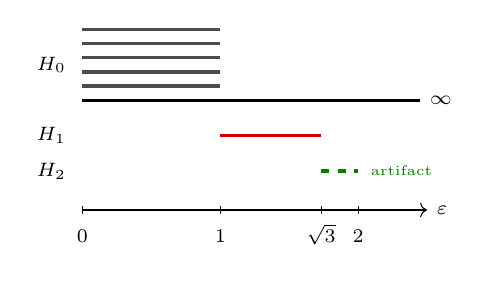
\begin{tikzpicture}[xscale=1.75,yscale=0.9]
  \draw[->] (0,-0.2)--(2.5,-0.2) node[right] {\scriptsize $\varepsilon$};
  \foreach \x/\lab in {0/0,1/1,1.732/\sqrt3,2/2}{
    \draw (\x,-0.15)--(\x,-0.25) node[below,text height=1.6ex] {\scriptsize $\lab$};}
  \node[left] at (-0.05,1.85) {\scriptsize $H_0$};
  \foreach \y in {1.55,1.75,1.95,2.15,2.35}{\draw[very thick,black!70] (0,\y)--(1,\y);}
  \draw[very thick,black] (0,1.35)--(2.45,1.35);
  \node[right] at (2.45,1.35) {\scriptsize $\infty$};
  \node[left] at (-0.05,0.85) {\scriptsize $H_1$};
  \draw[very thick,red!80!black] (1,0.85)--(1.732,0.85);
  \node[left] at (-0.05,0.35) {\scriptsize $H_2$};
  \draw[very thick,green!50!black,dashed] (1.732,0.35)--(2,0.35);
  \node[right,green!50!black] at (2.02,0.35) {\tiny artifact};
                \end{tikzpicture}
            \end{column}
        \end{columns}

        \vspace{0.4em}

        \begin{block}{You already know the $H_0$ half of this}
            The $H_0$ death times are exactly the merge heights of the \alert{single-linkage
            dendrogram}, i.e.\ the edge weights of a minimum spanning tree. Persistent homology
            \emph{is} hierarchical clustering in dimension $0$ --- and $H_1$, $H_2$ are the part
            you cannot get any other way.
        \end{block}
    \end{frame}

    \ifcomputedslides
    \begin{frame}{The hexagon, actually computed}
        \computedfig[0.51]{talk_04_persistence}{%
            The cloud, its barcode and its diagram. One $H_1$ bar, $[1,\sqrt3)$, and it is
            the only thing in the picture that is long. The script also checks the claim
            on the previous slide outright: the $H_0$ death times agree with the
            minimum-spanning-tree edge weights \emph{to machine precision} on a
            $60$-point cloud. The next slide reads off every number.}{talk\_04\_persistence.py}
    \end{frame}
    \fi

    \ifcomputedslides
    \begin{frame}[shrink=8]{The hexagon's diagram, number by number}
        \begin{columns}[T,onlytextwidth]
            \begin{column}{0.53\textwidth}
                \small
                {\footnotesize
                \begin{tabular}{@{}lll@{}}
                    \toprule
                    $\varepsilon$ & added & bars \\
                    \midrule
                    $0$ & $6$ vertices & $6\times H_0$ start \\
                    $1$ & $6$ sides & $5\times H_0$ end; $H_1$ starts \\
                    $\sqrt3$ & $6$ diagonals, $8$ triangles & $H_1$ ends; $H_2$ starts \\
                    $2$ & the rest & $H_2$ ends \\
                    \bottomrule
                \end{tabular}\par}

                \vspace{0.6em}
                Each bar $[b,d)$ becomes the point $(b,d)$ on the diagram:
                \begin{itemize}
                    \item $[0,1)$ five times $\to$ $(0,1)$, marked $\times5$;
                    \item $[0,\infty)$ $\to$ $(0,\infty)$, on the dashed line;
                    \item $[1,\sqrt3)$ $\to$ $(1,1.73)$: persistence $0.73$, \HL{the loop};
                    \item $[\sqrt3,2)$ $\to$ $(1.73,2)$: persistence $0.27$, the Rips artifact.
                \end{itemize}
            \end{column}
            \begin{column}{0.45\textwidth}
                \small
                \begin{block}{Six sides: five deaths and one birth}
                    Add the sides one at a time. Each of the first five joins two
                    different components: one $H_0$ bar ends. The sixth joins two vertices
                    that are \emph{already} connected, so it merges nothing and closes a
                    cycle instead: the $H_1$ bar starts.
                \end{block}
                \begin{alertblock}{Why one $H_0$ bar never ends}
                    Six components merging into one is $5$ deaths, not $6$. What is left is
                    the whole connected complex, and adding simplices can join components
                    but never remove the last one: $\beta_0\ge1$ forever. Which bar
                    survives is the elder rule; all were born at $0$, so the tie goes to
                    the vertex inserted first.
                \end{alertblock}
            \end{column}
        \end{columns}
    \end{frame}
    \fi

    \begin{frame}[shrink=5]{Distance between diagrams: the bottleneck distance}
        \begin{block}{Bottleneck distance $\dB(D,D')$}
            Match the points of $D$ with the points of $D'$ one to one, where any point may
            instead be matched to the diagonal (declared noise).
            \begin{itemize}
                \item Pair $(b,d)\leftrightarrow(b',d')$ costs
                $\max\bigl(|b-b'|,\,|d-d'|\bigr)$.
                \item Sending $(b,d)$ to the diagonal costs $(d-b)/2$, half its persistence.
            \end{itemize}
            $\dB$ is the smallest possible value of the \emph{largest} cost in a matching.
        \end{block}
        \small
        \textbf{Worked example.} $D=\{(1,1.73)\}$, the hexagon's loop;
        $D'=\{(1.1,1.65),\ (0.6,0.7)\}$.
        \begin{center}
            \footnotesize
            \begin{tabular}{@{}lll@{}}
                \toprule
                matching & costs & largest \\
                \midrule
                loop $\leftrightarrow(1.1,1.65)$, \ $(0.6,0.7)\to$ diagonal
                    & $0.1$, \ $0.05$ & \HL{$0.1$} \\
                everything to the diagonal & $0.37$, \ $0.28$, \ $0.05$ & $0.37$ \\
                loop $\leftrightarrow(0.6,0.7)$, \ $(1.1,1.65)\to$ diagonal
                    & $1.03$, \ $0.28$ & $1.03$ \\
                \bottomrule
            \end{tabular}
        \end{center}
        So $\dB(D,D')=0.1$: the loop moved by $0.1$, and the new point is noise.
        In general this is a bipartite matching problem (binary-search the threshold, test
        for a perfect matching). \textbf{Wasserstein} sums the costs instead:
        $W_2=\sqrt{0.1^2+0.05^2}\approx0.11$.

        \vspace{0.3em}
        \pause
        \centering Move one hexagon point $0.1$ outwards: $\dH=0.1$, the loop's bar
        becomes $[1.054,\sqrt3)$, and $\dB=0.054\le2\cdot0.1$. That inequality is the stability theorem, two slides on.
    \end{frame}

    \begin{frame}[shrink=5]{Bottleneck distance, precisely}
        \begin{columns}[T,onlytextwidth]
            \begin{column}{0.55\textwidth}
                \small
                \begin{block}{Definition}
                    Add the diagonal $\Delta=\{(t,t)\}$ to both diagrams, every point of it
                    available as often as needed. Then
                    \[
                        \dB(D,D')=\min_{\gamma}\ \max_{p}\ \|p-\gamma(p)\|_\infty ,
                    \]
                    over bijections $\gamma: D\cup\Delta\to D'\cup\Delta$.
                \end{block}
                \textbf{Why the diagonal.} Two diagrams rarely have the same number of
                points, and noise appears and disappears right next to the diagonal. A
                point with nothing to match is deleted by moving it there.

                \vspace{0.3em}
                \textbf{Why $\|\cdot\|_\infty$ and $(d-b)/2$.} Moving birth \emph{and}
                death by at most $\delta$ is a $\delta$-perturbation. The nearest diagonal
                point to $(b,d)$ is $\bigl(\tfrac{b+d}2,\tfrac{b+d}2\bigr)$, and both
                coordinates move by $\tfrac{d-b}2$.
            \end{column}
            \begin{column}{0.43\textwidth}
                \centering
                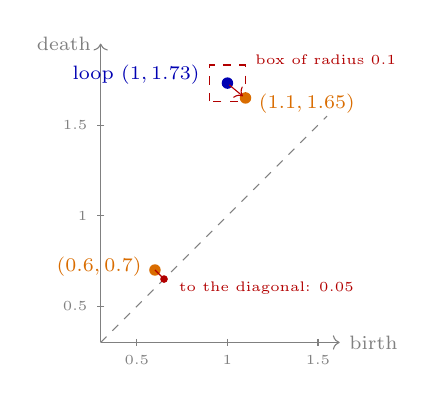
\begin{tikzpicture}[scale=2.3]
                    \draw[->,gray] (0.3,0.3) -- (1.62,0.3) node[right] {\scriptsize birth};
                    \draw[->,gray] (0.3,0.3) -- (0.3,1.95) node[left] {\scriptsize death};
                    \draw[gray,dashed] (0.3,0.3) -- (1.55,1.55);
                    \foreach \t in {0.5,1,1.5}{
                        \draw[gray] (\t,0.32)--(\t,0.28) node[below] {\tiny\t};}
                    \foreach \t in {0.5,1,1.5}{
                        \draw[gray] (0.32,\t)--(0.28,\t) node[left] {\tiny\t};}
                    \draw[red!70!black,dashed] (0.9,1.632) rectangle (1.1,1.832);
                    \fill[blue!70!black] (1,1.732) circle (0.9pt);
                    \node[blue!70!black,left] at (0.9,1.78) {\scriptsize loop $(1,1.73)$};
                    \fill[orange!85!black] (1.1,1.65) circle (0.9pt);
                    \node[orange!85!black,right] at (1.12,1.62) {\scriptsize $(1.1,1.65)$};
                    \draw[->,red!70!black] (1.01,1.722) -- (1.085,1.66);
                    \node[red!70!black,right] at (1.1,1.86) {\tiny box of radius $0.1$};
                    \fill[orange!85!black] (0.6,0.7) circle (0.9pt);
                    \fill[red!70!black] (0.65,0.65) circle (0.6pt);
                    \draw[red!70!black] (0.6,0.7) -- (0.65,0.65);
                    \node[orange!85!black,left] at (0.58,0.72) {\scriptsize $(0.6,0.7)$};
                    \node[red!70!black,right] at (0.68,0.6) {\tiny to the diagonal: $0.05$};
                \end{tikzpicture}

                \vspace{0.3em}
                \footnotesize\raggedright
                The best matching from the last slide: the moved point lies in the loop's
                $\|\cdot\|_\infty$-box of radius $0.1$, and the point near the diagonal is
                deleted for $0.05$. $\dB=0.1$.
            \end{column}
        \end{columns}
        \vspace{0.4em}
        \small
        \textbf{Points at infinity} (the $H_0$ bar that never dies) are matched only with
        each other, by birth: $[0,\infty)$ vs $[0.2,\infty)$ costs $0.2$. If the two
        diagrams have different numbers of them, $\dB=\infty$.
        \alert{Only the worst pair counts}: $\dB$ ignores many small changes; Wasserstein
        adds them up.
    \end{frame}

    \begin{frame}[shrink=5]{Computing the bottleneck distance}
        \begin{columns}[T,onlytextwidth]
            \begin{column}{0.5\textwidth}
                \small
                \textbf{1. Make it square.} Rows: the points of $D$, plus one diagonal slot
                per point of $D'$. Columns: the points of $D'$, plus one diagonal slot per
                point of $D$. A point may only go to \emph{its own} slot; slot to slot is
                free.
                \begin{center}
                    \footnotesize
                    \begin{tabular}{@{}l|ccc@{}}
                        & $(1.1,1.65)$ & $(0.6,0.7)$ & $\Delta_{\text{loop}}$ \\
                        \hline
                        loop $(1,1.73)$ & \HL{$0.1$} & $1.03$ & $0.37$ \\
                        $\Delta_{(1.1,1.65)}$ & $0.28$ & $\infty$ & \HL{$0$} \\
                        $\Delta_{(0.6,0.7)}$ & $\infty$ & \HL{$0.05$} & $0$ \\
                    \end{tabular}
                \end{center}
            \end{column}
            \begin{column}{0.48\textwidth}
                \small
                \textbf{2. Search the threshold.} The answer is one of the entries:
                $0,\ 0.05,\ 0.1,\ 0.28,\ 0.37,\ 1.03$. For a candidate $r$, keep the
                entries $\le r$ and ask: is there a perfect matching?
                \begin{itemize}
                    \item $r=0.05$: no --- the loop's row has nothing $\le0.05$.
                    \item $r=0.1$: yes --- the highlighted cells.
                \end{itemize}
                So $\dB=0.1$. Binary search over the sorted entries; each test is a
                bipartite matching (Hopcroft--Karp).
            \end{column}
        \end{columns}
        \vspace{0.5em}
        \small
        \textbf{3. Cost.} $n$ points give $O(n^2)$ candidates, so $O(\log n)$ matching tests,
        each $O(n^{2.5})$. Geometric tricks (Kerber--Morozov--Nigmetov 2017) make it fast for
        thousands of points: \texttt{persim}, \texttt{GUDHI}, \texttt{hera}.
        \alert{Wasserstein} swaps ``smallest largest cost'' for ``smallest total cost'': the
        same matrix, solved by the Hungarian algorithm.
    \end{frame}

    \begin{frame}[shrink=8]{Stability: why anyone trusts this}
        \begin{alertblock}{Stability, informally}
            Perturb the data a little and the diagram moves a little.
        \end{alertblock}

        \vspace{0.4em}
        \small
        Precisely: with $\dB$ the bottleneck distance (slides 40--42) and $\dH$ the
        Hausdorff distance (Part 2), for point clouds $X,Y$,
        \[
            \dB\bigl(\Dgm_k(X),\Dgm_k(Y)\bigr)\ \le\ 2\,\dH(X,Y),
        \]
        \HL{The diagram is a Lipschitz function of the data}, with constant $2$. \emph{(Cohen-Steiner--Edelsbrunner--Harer 2007; Chazal et al.)}

        \begin{block}{Lipschitz function}
            A map $f:(A,d)\to(A',d')$ between metric spaces is \emph{$K$-Lipschitz} if
            $d'\bigl(f(a),f(b)\bigr)\le K\,d(a,b)$ for all $a,b$: it never stretches a
            distance by more than a factor $K$. \ $x\mapsto2x$ is $2$-Lipschitz, $\sin$ is
            $1$-Lipschitz, $x\mapsto x^2$ on $\R$ is not Lipschitz (ever steeper).
            Here $f=\Dgm_k$, $d=\dH$, $d'=\dB$, $K=2$.
        \end{block}

        Three consequences worth stating out loud:
        \begin{itemize}
            \small
            \item Noise of size $\delta$ can only create bars of length $\le 2\delta$.
            \alert{This is the theorem behind ``long bars matter''.}
            \item You can bootstrap: resample, recompute, get a confidence band, keep only the
            points outside it --- the same instinct as a confidence interval on any
            other learned statistic.
            \item Diagrams estimated from a sample converge to the diagram of the underlying
            space. It is a statistic, not a picture.
        \end{itemize}
    \end{frame}

    \ifcomputedslides
    \begin{frame}{Stability, measured rather than quoted}
        \computedfig[0.52]{talk_04_stability}{%
            Right: the same circle perturbed at four noise levels, with $\dB(H_1)$ against
            the bound $2\,\dH$. The measured distance stays under the dashed line every
            time, with a factor of two or more to spare --- the theorem is a worst case,
            and Gaussian noise on a circle is not it. Left: the hexagon's Betti curves,
            for comparison.}{talk\_04\_persistence.py}
    \end{frame}
    \fi

    \begin{frame}{How it is computed (still linear algebra)}
        \small
        Order all $m$ simplices by insertion time and form the single boundary matrix
        $D$ ($D_{ij}=\pm1$ iff $\sigma_i$ is a facet of $\sigma_j$).
        For a nonzero column $j$, let $\mathrm{low}(j)$ be the row of its lowest nonzero.

        \begin{block}{Reduction}
            \scriptsize
            $R\leftarrow D$; \ \textbf{for} $j=1,\dots,m$: \ \textbf{while} some $j'<j$ has
            $\mathrm{low}(j')=\mathrm{low}(j)\neq0$: \ add column $j'$ to column $j$.
        \end{block}

        After reduction:
        \begin{itemize}
            \small
            \item $\mathrm{low}(j)=i$ $\Rightarrow$ a feature born with $\sigma_i$ dies with
            $\sigma_j$: the bar $[t_i,t_j)$.
            \item column $j$ zero and unpaired $\Rightarrow$ an infinite bar $[t_j,\infty)$.
        \end{itemize}

        \vspace{0.4em}

        It is left-to-right Gaussian elimination that never permutes columns.
        Worst case $O(m^3)$; in practice near-linear, thanks to clearing, cohomology
        duality, and never storing $D$ (Ripser).

        \vspace{0.4em}
        \begin{center}
            \alert{Same matrices as Part 3, one extra bookkeeping rule.}
        \end{center}
    \end{frame}

    \begin{frame}{Reading a diagram honestly}
        \small
        \begin{itemize}
            \item \textbf{Scale is not intrinsic.} Multiply all distances by $10$ and every bar
            gets $10\times$ longer. Compare persistences only after fixing a normalisation
            --- just as you would normalise features before $k$-NN.
            \item \textbf{Outliers are the enemy.} One far point changes $H_0$ and can manufacture
            loops. Trim by density, or use a distance-to-measure filtration, which is
            robust by construction.
            \item \textbf{Long does not always mean real.} Rips complexes generate their own
            artifacts. \emph{(Six points on a circle produce a genuine $H_2$ bar
                $[\sqrt3,2)$ --- the complex is combinatorially an octahedron boundary. The
                data has no void.)}
            \item \textbf{A diagram says a loop exists, not where it is.} Extracting a
            representative cycle is a separate, non-unique computation.
            \HL{Part 6 gives a canonical choice.}
        \end{itemize}
    \end{frame}

    \begin{frame}{Which bars are the shape?}
        \footnotesize
        \begin{columns}[T,onlytextwidth]
            \begin{column}{0.3\textwidth}
                \textbf{Margin.} Longest bar over the runner-up. Cheap, no guarantee.
            \end{column}
            \begin{column}{0.33\textwidth}
                \textbf{Null model.} Shuffle each coordinate: same marginals, no shape. Beat
                its $95$th percentile.
            \end{column}
            \begin{column}{0.33\textwidth}
                \textbf{Bootstrap band} \emph{(Fasy et al.\ 2014)}. Resample; $c$ = $95$th
                percentile of $\dB(\Dgm X,\Dgm X^*)$. Beat $2c$.
            \end{column}
        \end{columns}
        \computedfig[0.515]{talk_04_signal_vs_noise}{%
            A feature must sit above both lines. Only the loop does: $1.684$, against a null
            of $0.628$ and a band of $0.598$.}{talk\_04\_signal\_vs\_noise.py}
    \end{frame}

    \begin{frame}[shrink=5]{If nothing is stable}
        \small
        The blob: its longest $H_1$ bar ($0.32$) is inside the null ($0.49$) and inside the
        band ($0.57$). No feature survives. What we \emph{can} conclude:
        \begin{itemize}
            \item \textbf{At this sample size the data look like a structureless blob:} one
            component, no loops. That is a result --- and the case where PCA and clustering
            are the right tools.
            \item \textbf{It is an upper bound, not proof of absence:} no loop larger than
            $2c\approx0.57$ in the data's units. A smaller one may exist; more points shrink $c$.
            \item \textbf{Check the modelling choices first:} the metric (Part 2), outliers
            (trim, or a density-aware filtration), normalisation.
        \end{itemize}
        \begin{alertblock}{Two traps}
            \begin{itemize}
                \item \textbf{Automatic choices always answer.} The ``most stable scale'' of the
                blob is $\varepsilon=0.60$ with $\beta=(2,6)$. Test whatever it picks.
                \item \textbf{Pick a null that destroys what you test.} The clusters' $H_0$ gap
                ($1.31$) is \emph{inside} the shuffle null ($1.47$): shuffling each coordinate
                keeps the gap between the clusters. The bootstrap band ($0.78$) sees it.
            \end{itemize}
        \end{alertblock}
        \figcredit{talk\_04\_signal\_vs\_noise.py}
    \end{frame}

    \ifcomputedslides
    \begin{frame}{The three data sets from Part 1, answered}
        \computedfigside[0.62]{talk_01_motivation}{%
            Mean $0$ for all three, and covariances agreeing to within sampling error, so
            PCA splits the variance $0.55/0.45$, $0.53/0.47$, $0.56/0.44$ --- nothing to
            choose between them. A $k$-means silhouette then picks $k=3$ for all
            three, cutting the \emph{loop}, one connected piece, into three arcs. The diagrams settle it,
            scoring each by its longest bar over the runner-up: for (b) the longest
            $H_1$ bar is $73\times$ the next, for (c) the longest $H_0$ bar is
            $2.2\times$ --- clear, but a far smaller margin --- and (a) reaches neither
            ($1.4\times$ in $H_0$, $1.2\times$ in $H_1$).}{talk\_01\_motivation.py}
    \end{frame}
    \fi

    \section{Demo: TDA in an AI pipeline}

    \begin{frame}{The problem with feeding this to a model}
        A persistence diagram is a \emph{multiset} of points of varying cardinality.

        \vspace{0.4em}
        \begin{itemize}
            \item Not a vector: no addition, no scalar multiplication, no fixed dimension.
            \item $(\mathcal D,\dB)$ is a complete metric space but does not embed
            isometrically into a Hilbert space.
        \end{itemize}

        \vspace{0.6em}

        \begin{alertblock}{Consequence}
            You cannot hand a diagram to a linear layer, an SVM, or a transformer. You must
            \HL{vectorise} it first --- ideally with a map that is Lipschitz in $\dB$, so the
            stability guarantee survives into feature space.
        \end{alertblock}
    \end{frame}

    \begin{frame}{Vectorisations}
        \small
        \begin{block}{Betti curve}
            $t\mapsto\beta_k(t)=\#\{i:b_i\le t<d_i\}$. Cheapest option; not Lipschitz in
            $\ell_\infty$, but a fine baseline feature.
        \end{block}
        \begin{block}{Persistence landscape (Bubenik 2015)}
            Tent functions $\Lambda_i(t)=\max(0,\min(t-b_i,d_i-t))$ ranked at each $t$; lives in
            an $L^p$ space, is $1$-Lipschitz in $\dB$, so means and hypothesis tests are well
            defined --- you can average landscapes across a batch the way you average anything else.
        \end{block}
        \begin{block}{Persistence image (Adams et al.\ 2017)}
            Map $(b,d)\mapsto(b,d-b)$, place a weighted Gaussian at each point, discretise on a
            grid. Fixed-size image output --- a direct CNN input, and the standard choice in
            recent \HL{topological deep learning} pipelines.
        \end{block}
        \begin{block}{Kernels}
            Sliced-Wasserstein and persistence-Fisher kernels plug straight into an SVM or a
            Gaussian process.
        \end{block}
    \end{frame}

    \ifcomputedslides
    \begin{frame}{One diagram, three vectorisations, and a null model}
        \computedfigside[0.64]{talk_05_pipeline}{%
            A noisy circle, its diagram, and that diagram as a Betti curve, a landscape
            and an image --- $60$, $240$ and $256$ numbers, fixed sizes whatever the
            diagram held. Bottom right: the observed loop against $20$ coordinate-shuffled
            replicates of it, which it clears by $3.2\times$.}{talk\_05\_pipeline.py}
    \end{frame}
    \fi

    \begin{frame}{A typical pipeline}
        \begin{center}
            \resizebox{0.98\textwidth}{!}{%
                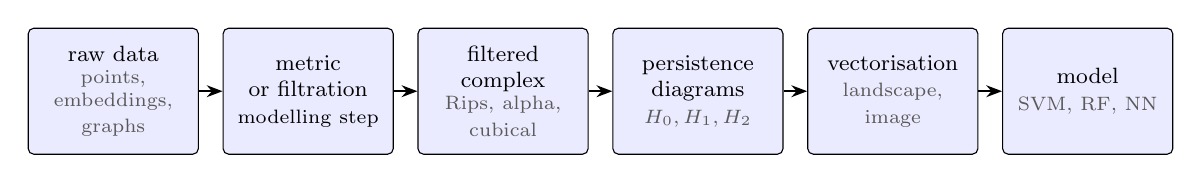
\begin{tikzpicture}[
                    node distance=0.45cm and 0.3cm,
                    box/.style={draw,rounded corners=2pt,align=center,inner sep=3pt,
                    minimum height=1.6cm,text width=1.95cm,font=\footnotesize,fill=blue!8},
                    arr/.style={-{Stealth[length=2mm]},thick}]
\node[box] (a) {raw data\\{\scriptsize\color{black!65} points,\\embeddings,\\graphs}};
\node[box,right=of a] (b) {metric\\or filtration\\{\scriptsize \alert{modelling step}}};
\node[box,right=of b] (c) {filtered\\complex\\{\scriptsize\color{black!65} Rips, alpha,\\cubical}};
\node[box,right=of c] (d) {persistence\\diagrams\\{\scriptsize\color{black!65} $H_0,H_1,H_2$}};
\node[box,right=of d] (e) {vectorisation\\{\scriptsize\color{black!65} landscape, image}};
\node[box,right=of e] (f) {model\\{\scriptsize\color{black!65} SVM, RF, NN}};
\foreach \x/\y in {a/b,b/c,c/d,d/e,e/f}{\draw[arr] (\x)--(\y);}
                \end{tikzpicture}}
        \end{center}

        \vspace{0.6em}
        \begin{itemize}
            \item Every stage after the metric is essentially parameter-free.
            \item Topological features are usually \HL{complementary}, not a replacement:
            concatenate them with your existing features and measure the lift.
            \item Cross-validate honestly: the diagram computation must sit \emph{inside}
            the CV loop if any preprocessing is data-dependent.
        \end{itemize}
    \end{frame}

    \begin{frame}{What TDA looks like inside an AI research pipeline}
        \small
        \begin{itemize}
            \item \textbf{Sanity-check the manifold hypothesis.} Persistent $H_0$/$H_1$ of a
            learned embedding tells you how many clusters and loops it actually has ---
            before you trust a downstream linear probe.
            \item \textbf{Diagnose generative models.} Track $\beta_0$ of generated samples
            across training to catch mode collapse; compare periodicity ($H_1$
            persistence) of real vs.\ generated trajectories.
            \item \textbf{OOD / robustness.} Score a new point by how it perturbs the
            persistence diagram of the training manifold, or by distance-to-measure ---
            both are stable by the theorem two slides ago.
            \item \textbf{Interpretability.} \HL{Mapper} covers the embedding by a lens
            function (density, a PCA coordinate, a target variable), clusters each
            preimage, and connects clusters that share points. The result is a graph
            summary of a hidden layer --- a complement to UMAP/t-SNE that keeps
            branching structure explicit instead of flattening it into 2D.
            \item \textbf{Beyond graphs.} Simplicial and cell complexes extend message passing
            to higher-order relations --- the subject of Part 6's closing slide.
        \end{itemize}
        \vspace{0.3em}

        \begin{center}
            \alert{Always compare against a null model} (shuffled data, Gaussian noise) before
            trusting a bar.
        \end{center}
    \end{frame}

    \section{The Hodge Laplacian}

    \begin{frame}{Redeeming the promise from Part 3}
        So far $\partial_k$ was a map. Give $C_k=\R^{n_k}$ its standard inner product ---
        declare the simplices an orthonormal basis. Then $\partial_k$ has an adjoint, and it
        is simply the transpose:
        \[
            \partial_k^{\mathsf T} : C_{k-1}\to C_k,
            \qquad \langle \partial_k x,\,y\rangle = \langle x,\,\partial_k^{\mathsf T} y\rangle .
        \]
        $\partial_k^{\mathsf T}$ is the \HL{coboundary}: it sends a simplex to the signed sum
        of the simplices having it as a face.

        \vspace{0.8em}

        \begin{block}{The Hodge (combinatorial) Laplacian}
            \[
                \boxed{\ L_k \;=\; \underbrace{\partial_k^{\mathsf T}\partial_k}_{\text{down}}
                    \;+\; \underbrace{\partial_{k+1}\partial_{k+1}^{\mathsf T}}_{\text{up}}\ }
                \qquad L_k : C_k\to C_k .
            \]
        \end{block}
        Symmetric, positive semidefinite, sparse. \HL{$L_0=\partial_1\partial_1^{\mathsf T}$
            is exactly the graph Laplacian $D-A$ from Part 3} --- the promise, kept.
    \end{frame}

    \begin{frame}[shrink=20]{The kernel is the homology}
        \begin{block}{One-line computation}
            For any $x\in C_k$,
            \[
                x^{\mathsf T}L_k x = \|\partial_k x\|^2 + \|\partial_{k+1}^{\mathsf T}x\|^2 .
            \]
            So $L_kx=0 \iff \partial_kx=0$ \emph{and} $\partial_{k+1}^{\mathsf T}x=0$.
        \end{block}
        Such $x$ are called \HL{harmonic}. They are the cycles that are also orthogonal to
        every boundary.

        \vspace{0.6em}

        \begin{block}{Hodge decomposition}
            \[
                C_k \;=\; \underbrace{\im\partial_{k+1}}_{\text{boundaries}}\ \oplus\
                \underbrace{\ker L_k}_{\text{harmonic}}\ \oplus\
                \underbrace{\im\partial_k^{\mathsf T}}_{\text{co-boundaries}} ,
            \]
            an orthogonal direct sum, and $\ker\partial_k=\im\partial_{k+1}\oplus\ker L_k$.
        \end{block}

        \vspace{0.3em}
        \begin{alertblock}{Consequence}
            \[
                \ker L_k \;\cong\; Z_k/B_k \;=\; H_k,
                \qquad\text{so}\qquad
                \boxed{\ \beta_k=\dim\ker L_k\ }.
            \]
            \centering \HL{Counting holes is finding the multiplicity of the eigenvalue $0$ ---
            same spectral-clustering fact as Part 3, one level up.}
        \end{alertblock}
    \end{frame}

    \begin{frame}[shrink=12]{Back to the triangle}
        Same $\partial_1,\partial_2$ as in Part 3. Multiply them out:

        \vspace{0.4em}
        \begin{columns}[T,onlytextwidth]
            \begin{column}{0.48\textwidth}
                \small
                \[
                    L_0=\partial_1\partial_1^{\mathsf T}=
                    \begin{pmatrix}
                        2&-1&-1\\ -1&2&-1\\ -1&-1&2
                    \end{pmatrix}
                \]
                Spectrum $\{0,3,3\}$: $\ \dim\ker L_0=1=\beta_0$. \checkmark

                \vspace{0.3em}
                {\scriptsize (This is the graph Laplacian of the triangle graph, $3I-J$.)}
            \end{column}
            \begin{column}{0.48\textwidth}
                \small
                \emph{Hollow} ($\partial_2=0$):
                \[
                    L_1=\partial_1^{\mathsf T}\partial_1=
                    \begin{pmatrix}
                        2&-1&1\\ -1&2&1\\ 1&1&2
                    \end{pmatrix}
                \]
                Spectrum $\{0,3,3\}$: $\ \dim\ker L_1=1=\beta_1$. \checkmark

                The harmonic vector is $(1,1,-1)^{\mathsf T}=z$.
            \end{column}
        \end{columns}

        \vspace{0.6em}

        \emph{Filled}: add $\partial_2\partial_2^{\mathsf T}$ with $\partial_2=(1,1,-1)^{\mathsf T}$:
        \[
            L_1=\begin{pmatrix}
                    2&-1&1\\ -1&2&1\\ 1&1&2
            \end{pmatrix}
            +\begin{pmatrix}
                 1&1&-1\\ 1&1&-1\\ -1&-1&1
            \end{pmatrix}
            =3I,
            \qquad \text{spectrum }\{3,3,3\},\quad \dim\ker L_1=0=\beta_1 . \ \checkmark
        \]
        \begin{center}
            \alert{Filling the triangle pushed the zero eigenvalue up to $3$.}
        \end{center}
    \end{frame}

    \ifcomputedslides
    \begin{frame}{\emph{Where} is the loop? The harmonic answer}
        \computedfig[0.50]{talk_06_hodge_laplacian}{%
            Left: the harmonic chain of a hexagon, drawn as a flow --- every edge carries
            the same weight, because nothing distinguishes them. Middle: a filled triangle
            with a two-edge bridge, where the single loop has two homologous routes home
            and the harmonic chain splits $2/3$ to $1/3$ between them. \alert{No barcode
            contains that.} Right: subdivide a cycle and $\beta_1$ never moves while the
            spectral gap does.}{talk\_06\_hodge\_laplacian.py}
    \end{frame}
    \fi

    \begin{frame}{Quick check: the spectrum sees more than $\beta_k$ does}
        \small
        \begin{enumerate}
            \item \textbf{Path graph on 3 vertices, $1$--$2$--$3$.} Write $\partial_1$
            ($2$ edges), form $L_0=\partial_1\partial_1^{\mathsf T}$, and check its
            spectrum is $\{0,1,3\}$: $\dim\ker L_0=1$ component, as expected.
            \item \textbf{Subdivide, and watch what does \emph{not} change.} Take the hollow
            triangle ($\beta_1=1$, spectrum $\{0,3,3\}$ above) and subdivide each edge
            once, so it is now a hexagon (still hollow, $6$ edges, no triangles).
            $\beta_1$ is still $1$ --- same one loop. But the spectrum moves:
            \[
                \{0,3,3\}\ \longrightarrow\ \{0,1,1,3,3,4\},
                \qquad \lambda_1(L_1):\ 3\ \to\ 1\ \to\ 0.268\ \text{(subdivide again)}.
            \]
        \end{enumerate}

        \vspace{0.5em}

        \begin{alertblock}{The point}
            $\beta_k$ only reads the eigenvalue $0$. The spectral gap $\lambda_1(L_k)$ is a
            Cheeger-type quantity that keeps changing with the mesh even while $\beta_k$ sits
            still --- two complexes can share a persistence diagram and have very different
            spectra. The diagram is a coarsening of the Laplacian, not the other way around.
        \end{alertblock}
    \end{frame}

    \begin{frame}[shrink=12]{Why this matters for AI research specifically}
        \small
        \begin{enumerate}
            \item \textbf{Canonical representatives.} $\ker L_k$ is a genuine subspace, not a
            quotient: each homology class has a unique minimum-norm harmonic
            representative --- the principled answer to ``\emph{where} is the loop?'',
            which the barcode alone does not give.
            \item \textbf{An eigensolver, not a column reduction.} $\beta_k$ via sparse
            symmetric eigensolvers (Lanczos), the same numerical stack you already use
            for spectral clustering --- and it is differentiable, unlike matrix reduction.
            \item \textbf{HodgeRank.} Ranking from inconsistent pairwise comparisons decomposes
            exactly along $C_1=\im\partial_1^{\mathsf T}\oplus\ker L_1\oplus\im\partial_2$:
            a global ranking, a genuinely cyclic (irreconcilable) part, and a local
            inconsistency part. \emph{(Jiang, Lim, Yao, Ye 2011.)}
            \item \textbf{Simplicial \& topological neural networks.} $L_k$ (and its persistent
            version) is the natural convolution operator once your data has higher-order
            relations, not just edges. \emph{(Ebli et al.\ 2020; Bunch et al.\ 2020;
            Bodnar et al., ``Weisfeiler and Lehman Go Topological'', 2021; Hajij et al.,
                ``Topological Deep Learning'', 2023, survey.)}
            \item \textbf{Persistent Laplacian.} For $K\subseteq L$ in a filtration,
            $L_k^{K,L}$'s kernel dimension recovers the persistent Betti number, plus a
            continuously varying nonzero spectrum the barcode discards.
            \emph{(Wang--Nguyen--Wei 2020; M\'emoli--Wan--Wang 2022, stability.)}
        \end{enumerate}
    \end{frame}

    \section{Wrap-up \& exercise}

    \begin{frame}[shrink=5]{Summary}
        \begin{block}{The pipeline}
            \centering
            point cloud / embedding $\to$ Rips filtration $\to$ boundary matrices $\to$ barcode
            $\;\;\big|\;\;$ Laplacian $\to$ spectrum
        \end{block}

        \vspace{0.5em}
        \small
        \begin{itemize}
            \item A scale $\varepsilon$ turns points into a simplicial complex.
            \item \HL{Chains are vectors, $\partial_k$ is a matrix, $\partial_k\partial_{k+1}=0$,
                and $\beta_k=\nullity\partial_k-\rank\partial_{k+1}$.} That is all of homology.
            \item Persistence removes the choice of $\varepsilon$ and returns a barcode;
            stability makes the barcode a Lipschitz function of the data, so it is a
            statistic you can do inference with and feed to a model.
            \item \HL{$L_k=\partial_k^{\mathsf T}\partial_k+\partial_{k+1}\partial_{k+1}^{\mathsf T}$
                and $\beta_k=\dim\ker L_k$}: the graph Laplacian behind spectral clustering
            and GCNs, generalised one level at a time, with strictly more information in
            the nonzero spectrum than the diagram alone carries.
        \end{itemize}

        \vspace{0.4em}

        \begin{alertblock}{Honest closing note}
            TDA is a complement to your toolbox, strongest when the phenomenon really is about
            connectivity, loops or branching. It is not a general-purpose accuracy boost, and it
            will not replace a well-tuned baseline on its own.
        \end{alertblock}
    \end{frame}

    \begin{frame}{Exercise}
        \begin{columns}[T,onlytextwidth]
            \begin{column}{0.36\textwidth}
                \centering
                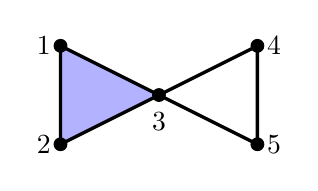
\begin{tikzpicture}[scale=1.25]
  \coordinate (v1) at (0,1);
  \coordinate (v2) at (0,0);
  \coordinate (v3) at (1,0.5);
  \coordinate (v4) at (2,1);
  \coordinate (v5) at (2,0);
  \fill[blue!30] (v1)--(v2)--(v3)--cycle;
  \draw[very thick] (v1)--(v2)--(v3)--cycle;
  \draw[very thick] (v3)--(v4)--(v5)--cycle;
  \foreach \p in {v1,v2,v3,v4,v5}{\fill (\p) circle (2pt);}
  \node[left] at (v1) {$1$}; \node[left] at (v2) {$2$};
  \node[below=3pt] at (v3) {$3$}; \node[right] at (v4) {$4$}; \node[right] at (v5) {$5$};
                \end{tikzpicture}
            \end{column}
            \begin{column}{0.60\textwidth}
                \small
                $K$ has vertices $1,2,3,4,5$; edges
                $12,\ 23,\ 13,\ 34,\ 45,\ 35$; and \alert{one} triangle, $123$
                (shaded). The right-hand triangle is \alert{not} filled.

                \vspace{0.6em}
                \begin{enumerate}
                    \item Write down $\partial_1$ ($5\times6$) and $\partial_2$ ($6\times1$).
                    \item Check $\partial_1\partial_2=0$.
                    \item Compute $\rank\partial_1$ and $\rank\partial_2$.
                    \item Give $\beta_0$ and $\beta_1$.
                    \item Verify with the Euler characteristic.
                \end{enumerate}

                \vspace{0.5em}

                \footnotesize
                \textbf{Answers.} $\rank\partial_1=4$, $\rank\partial_2=1$;
                $\beta_0=5-4=1$, $\beta_1=(6-4)-1=1$.
                Euler: $5-6+1=0=\beta_0-\beta_1$. \checkmark
                The filled triangle contributes no hole; the empty one does.
            \end{column}
        \end{columns}
    \end{frame}

    \ifcomputedslides
    \begin{frame}{The exercise, checked --- and both halves of the talk agreeing}
        \computedfig[0.54]{talk_07_exercise}{%
            Left: the complex you just did by hand. Middle: its harmonic loop, which is
            non-zero on $34$, $45$, $35$ and \emph{exactly zero} on the filled triangle
            --- Part 6 locating the hole that Part 3 only counted. Right: the appendix
            figure-eight as a point cloud, where the Rips pipeline recovers
            $\beta_1=2$ from nothing but pairwise
            distances.}{talk\_07\_exercise.py}
    \end{frame}
    \fi

    \begin{frame}[shrink=10]{Where to go next}
        \scriptsize
        \begin{block}{Classic TDA}
            \begin{itemize}
                \item Edelsbrunner \& Harer, \emph{Computational Topology: An Introduction} (2010).
                \item Dey \& Wang, \emph{Computational Topology for Data Analysis} (2022) --- modern, algorithmic.
                \item Carlsson, ``Topology and Data'', \emph{Bull.\ AMS} 46 (2009).
                \item Cohen-Steiner, Edelsbrunner, Harer, ``Stability of Persistence Diagrams'' (2007).
                \item Chazal \& Michel, ``An Introduction to TDA for Statisticians'' (2021).
            \end{itemize}
        \end{block}
        \begin{block}{Hodge theory and topological deep learning}
            \begin{itemize}
                \item Eckmann, ``Harmonische Funktionen und Randwertaufgaben in einem Komplex'' (1944) --- the original combinatorial Hodge theory.
                \item Jiang, Lim, Yao, Ye, ``Statistical ranking and combinatorial Hodge theory'' (2011).
                \item Wang, Nguyen, Wei, ``Persistent spectral graph'' (2020); M\'emoli, Wan, Wang, ``Persistent Laplacians'' (2022).
                \item Bodnar et al., ``Weisfeiler and Lehman Go Topological: Message Passing Simplicial Networks'' (2021).
                \item Hajij et al., ``Topological Deep Learning: Going Beyond Graph Data'' (2023) --- broad survey, good starting point.
                \item Bronstein et al., ``Geometric Deep Learning'' (2021) --- for the surrounding context.
            \end{itemize}
        \end{block}
        \begin{block}{Code}
            \texttt{pip install ripser persim gudhi giotto-tda} --- then reproduce today's hexagon,
            and run the Rips pipeline on one of your own embeddings.

            \vspace{0.3em}
            Every computed figure in this deck comes from the accompanying repository, which
            implements the filtration, the reduction and the Hodge Laplacian from scratch in
            NumPy. \texttt{python run\_examples.py -{}-talk} regenerates all of them and
            re-checks, part by part, the numbers claimed on these slides.
        \end{block}
    \end{frame}

    \begin{frame}[standout]
  Questions?
    \end{frame}

    \appendix

    \begin{frame}{Appendix: going further}
        \small
        The figure-eight --- two loops sharing a vertex, $\beta_1=2$ --- is worked in the
        right-hand panel of the exercise check, both as an abstract complex and from a point
        cloud, using nothing but pairwise distances.

        \vspace{0.6em}
        \begin{block}{Take-home problem}
            Take an embedding you already have (sentence embeddings, a hidden layer, a t-SNE
            input \emph{before} projection) and run the Rips pipeline from Part 5 on it, for
            example with \texttt{ripser}.
            Compare the $H_1$ barcode of the real data against a Gaussian-noise baseline of the
            same size and dimension. Is there a bar that clearly survives the comparison?
        \end{block}
    \end{frame}

\end{document}
